Una gráfica $G = (V, E)$ consiste en un conjunto de \textbf{vértices} $V$ y un conjunto de \textbf{aristas} $E \subseteq \binom{V}{2}$. Partimos de las nociones elementales de vecindad, grado, caminos, ciclos y conectividad, sin repetirlas aquí. Esta sección se enfoca en resultados matemáticos que fundamentan el resto del capítulo y que raramente se ven en cursos de computación.
\\\\
Existen dos representaciones estándar de una gráfica, con complejidades muy distintas:
\begin{itemize}
    \item \textbf{Lista de adyacencia}: conviene cuando el grafo es \emph{disperso}, es decir, cuando $E \ll V^2$.
    \item \textbf{Matriz de adyacencia}: conviene cuando se necesitan consultas de aristas en $O(1)$, o cuando $V$ es pequeño ($V \leq 500$) y ese costo de espacio es aceptable.
\end{itemize}
La tabla resume las operaciones más frecuentes en cada representación.

\begin{table}[H]
\centering
\renewcommand{\arraystretch}{1.4}
\begin{tabular}{lll}
\toprule
\textbf{Operación} & \textbf{Lista de adyacencia} & \textbf{Matriz de adyacencia} \\
\midrule
Espacio                    & $O(V + E)$  & $O(V^2)$ \\
¿Existe arista $(u,v)$?    & $O(\deg u)$ & $O(1)$ \\
Vecinos de $u$             & $O(\deg u)$ & $O(V)$ \\
Agregar arista             & $O(1)$      & $O(1)$ \\
\bottomrule
\end{tabular}
\end{table}
\section{Lema de los apretones de mano}
Si en una reunión cada persona estrecha la mano con algunos asistentes, podemos contar las ``manos involucradas'' de dos formas: sumando cuántas veces saludó cada persona, o bien contando cada apretón dos veces (una por cada extremo). El lema traduce esa idea a grafos: cada arista aporta $1$ al grado de cada uno de sus dos extremos.
\\\\
En todo grafo $G = (V, E)$:
\[
\sum_{v \in V} \deg(v) = 2|E|
\]

$Demostración$. Cada arista $\{u, v\}$ contribuye exactamente $1$ al grado de $u$ y $1$ al grado de $v$, es decir, contribuye $2$ a la suma total de grados. Sumando sobre todas las aristas: $\sum_v \deg(v) = 2|E|$. 

En todo grafo, el número de vértices de grado impar es par.
\\\\
$Demostración$.
Sea $I$ el conjunto de vértices de grado impar y $P$ el de grado par. Entonces:
\[
2|E| = \sum_{v \in I} \deg(v) + \sum_{v \in P} \deg(v)
\]
El segundo término es par (suma de números pares). Como $2|E|$ es par, el primer término también debe serlo.
\\\\
Este corolario tiene consecuencias sorprendentes en el ICPC. Por ejemplo: en un torneo (grafo dirigido completo), la suma de grados de salida es $\binom{n}{2}$; argumentos de paridad sobre los grados pueden determinar si cierta configuración es posible sin necesidad de construirla.

\section{Caminos y circuitos de Euler}
\subsection*{Los puentes de Königsberg}
En 1736, Leonhard Euler resolvió el siguiente problema planteado por los habitantes de la ciudad de Königsberg. La ciudad tenía 7 puentes que conectaban 4 zonas de tierra. ¿Es posible dar un paseo cruzando cada puente exactamente una vez y regresar al punto de partida?
\begin{figure}[H]
\centering
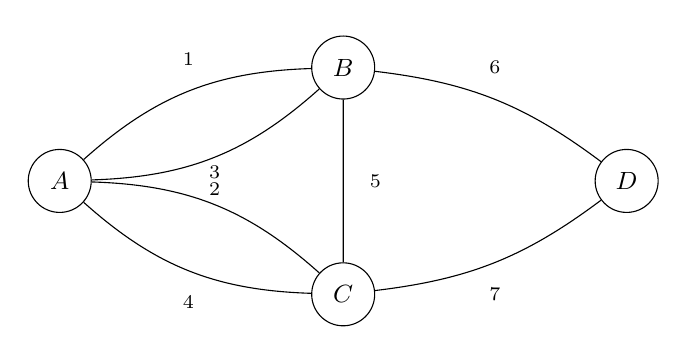
\begin{tikzpicture}[
  every node/.style={circle,draw,minimum size=0.8cm,font=\small},
  scale=1.2
]
  \node (A) at (0, 0)    {$A$};
  \node (B) at (3, 1.2)  {$B$};
  \node (C) at (3,-1.2)  {$C$};
  \node (D) at (6, 0)    {$D$};
 
  \draw (A) to[bend left=20]  node[draw=none,above,font=\scriptsize]{1}(B);
  \draw (A) to[bend right=20] node[draw=none,below,font=\scriptsize]{2}(B);
  \draw (A) to[bend left=20]  node[draw=none,above,font=\scriptsize]{3}(C);
  \draw (A) to[bend right=20] node[draw=none,below,font=\scriptsize]{4}(C);
  \draw (B) --                node[draw=none,right,font=\scriptsize]{5}(C);
  \draw (B) to[bend left=15]  node[draw=none,above,font=\scriptsize]{6}(D);
  \draw (C) to[bend right=15] node[draw=none,below,font=\scriptsize]{7}(D);
\end{tikzpicture}
\end{figure}
 
Euler demostró que tal paseo es \textbf{imposible} y al hacerlo fundó
la teoría de gráficas. Su argumento fue que cada vez que el paseo pasa por una
zona (sin empezar ni terminar ahí), usa un puente para entrar y otro
para salir. Por lo tanto esa zona debe tener un número par de puentes.
Las zonas $B$ y $C$ tienen 3 puentes cada una, así que el paseo
no puede existir.
 
\begin{definition}[Camino y circuito euleriano]
En una gráfica $G$:
\begin{itemize}
    \item Un \textbf{camino euleriano} es un camino que recorre cada
          arista exactamente una vez.
    \item Un \textbf{circuito euleriano} es un camino euleriano que
          empieza y termina en el mismo vértice.
    \item $G$ es \textbf{euleriano} si tiene un circuito euleriano.
\end{itemize}
\end{definition}
 
Sea $G$ conexa. Entonces:
\begin{itemize}
    \item $G$ tiene un \textbf{circuito euleriano} si y solo si todo
          vértice tiene grado par.
    \item $G$ tiene un \textbf{camino euleriano} (no circuito) si y solo
          si exactamente dos vértices tienen grado impar, y el camino
          debe empezar en uno de ellos y terminar en el otro.
\end{itemize}
\subsection{Algoritmo de Hierholzer}
 
Verificar si existe un circuito euleriano es fácil. Encontrarlo es lo que requiere el algoritmo de Hierholzer.
\\\\
Intuitivamente, el algoritmo parte de cualquier vértice y sigue aristas arbitrarias hasta regresar al punto de partida. Esto va a formar un circuito, pero puede no ser euleriano. Si algún vértice del circuito actual tiene aristas sin usar, se extiende el circuito
desde ese vértice. Se repite esto hasta usar todas las aristas.
 
\begin{lstlisting}[language=C++]
// Hierholzer: construye un circuito euleriano desde 'inicio'.
// Asume que adj[v] es la lista de vecinos (se consume al recorrer).
vector<int> hierholzer(int inicio) {
    stack<int> st;
    vector<int> circuito;
    st.push(inicio);

    while (!st.empty()) {
        int v = st.top();

        if (adj[v].empty()) {
            // No quedan aristas salientes: v entra al circuito.
            circuito.push_back(v);
            st.pop();
        } else {
            // Tomamos una arista v -> u y seguimos el recorrido.
            int u = adj[v].back();
            adj[v].pop_back();
            st.push(u);
        }
    }

    reverse(circuito.begin(), circuito.end());
    return circuito;
}
\end{lstlisting}
Muchos problemas se reducen a encontrar un camino o circuito euleriano
de forma no obvia. El patrón general es construir un grafo donde lo
que se quiere recorrer son las \textbf{aristas}, no los vértices. Imaginemos que nos dan
un conjunto de palabras y nos preguntan, ¿es posible ordenarlas en una secuencia tal que la última letra de cada palabra sea la primera de la siguiente? Podemos modelar cada letra como un vértice, cada palabra como una arista dirigida de su primera letra a su última. La
secuencia existe si y solo si el grafo tiene un camino euleriano.
\section{Componentes fuertemente conexas}
En un grafo \textbf{no dirigido}, la conectividad es simple, hay un
camino entre dos nodos o no. Pero en un grafo \textbf{dirigido} la
situación es más complicada, pues puede haber un camino de $u$ a $v$ sin que
haya uno de $v$ a $u$.
 
\begin{definition}
Una \textbf{componente fuertemente conexa} (SCC) de una gráfica dirigida
es un subconjunto maximo de vértices $C$ tal que para todo par
$u, v \in C$ existe un camino de $u$ a $v$ y un camino de $v$ a $u$.
\end{definition}
\subsection{Algoritmo de Kosaraju}
El algoritmo de Kosaraju encuentra todas las SCCs en $O(V + E)$ con dos DFS. Se apoya en el \textbf{grafo transpuesto} $G^T$ (mismos nodos, aristas invertidas). Las SCCs de $G$ y $G^T$ son las mismas, aunque cambia el orden en que conviene descubrirlas.
\\\\
El procedimiento tiene dos pasos:
\begin{enumerate}
    \item \textbf{DFS en $G$.} Al terminar de explorar cada nodo, lo añadimos al final de una lista \texttt{order}. Un nodo se registra tarde cuando aún quedaban descendientes por visitar; por eso el último de la lista pertenece a una SCC sin aristas entrantes desde otras componentes.
    \item \textbf{DFS en $G^T$, en orden inverso.} Recorremos \texttt{order} de atrás hacia adelante. Cada vez que encontramos un nodo sin componente asignada, lanzamos un DFS en $G^T$ desde ahí. Ese DFS descubre \emph{exactamente} una SCC: en $G^T$ las aristas que salían hacia otras componentes se volvieron entradas, así que no podemos salir de la componente actual.
\end{enumerate}
 
\begin{figure}[H]
\centering
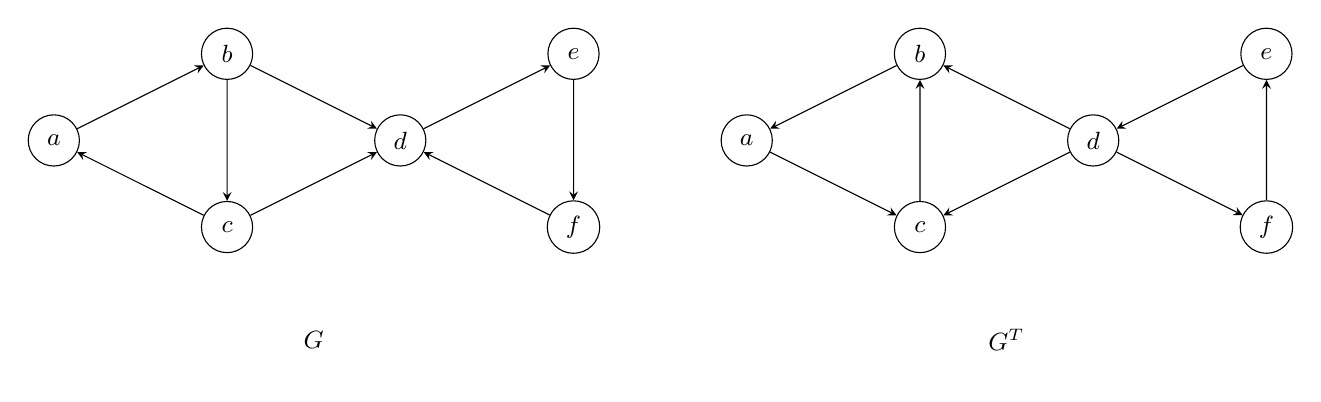
\begin{tikzpicture}[
  every node/.style={circle,draw,minimum size=0.65cm,font=\small},
  scale=1.1
]
  \begin{scope}[->, >=stealth]
    \node (a) at (0,2)   {$a$};
    \node (b) at (2,3)   {$b$};
    \node (c) at (2,1)   {$c$};
    \node (d) at (4,2)   {$d$};
    \node (e) at (6,3)   {$e$};
    \node (f) at (6,1)   {$f$};
    \draw (a)--(b); \draw (b)--(c); \draw (c)--(a);
    \draw (b)--(d); \draw (c)--(d);
    \draw (d)--(e); \draw (e)--(f); \draw (f)--(d);
    \node[draw=none,font=\small] at (3,-0.3) {$G$};
  \end{scope}
 
  \begin{scope}[xshift=8cm, ->, >=stealth]
    \node (a2) at (0,2)  {$a$};
    \node (b2) at (2,3)  {$b$};
    \node (c2) at (2,1)  {$c$};
    \node (d2) at (4,2)  {$d$};
    \node (e2) at (6,3)  {$e$};
    \node (f2) at (6,1)  {$f$};
    \draw (b2)--(a2); \draw (c2)--(b2); \draw (a2)--(c2);
    \draw (d2)--(b2); \draw (d2)--(c2);
    \draw (e2)--(d2); \draw (f2)--(e2); \draw (d2)--(f2);
    \node[draw=none,font=\small] at (3,-0.3) {$G^T$};
  \end{scope}
\end{tikzpicture}
\end{figure}
 
En el ejemplo de la figura las SCCs son $\{a,b,c\}$ y $\{d,e,f\}$. Veamos el algoritmo paso a paso suponiendo que los nodos se numeran $a=0,b=1,c=2,d=3,e=4,f=5$ y que el primer DFS recorre $G$ en ese orden.

\textbf{Paso 1 (DFS en $G$).} Empezamos en $a$: visitamos $a \to b \to c$; desde $c$ seguimos a $d$, luego $d \to e \to f$, y al retroceder registramos cada nodo al terminar:
\[
\texttt{order} = [f,\, e,\, d,\, c,\, b,\, a].
\]
El último en la lista es $a$, de la componente $\{a,b,c\}$. Intuitivamente, al explorar desde $a$ ``empujamos'' todo el triángulo $\{d,e,f\}$ antes de cerrar $a$.

\textbf{Paso 2 (DFS en $G^T$, orden inverso).} Procesamos \texttt{order} de derecha a izquierda:
\begin{itemize}
    \item Desde $a$ (primero en este orden): en $G^T$ solo podemos retroceder por aristas invertidas dentro de $\{a,b,c\}$ (ciclo $a \to c \to b \to a$). Las flechas $b \to d$ y $c \to d$ de $G$ se vuelven $d \to b$ y $d \to c$ en $G^T$, pero $d$ aún no se visita desde $a$ porque esas aristas \emph{entran} a $\{a,b,c\}$, no salen de $a$. Resultado: $\{a,b,c\}$ recibe \texttt{comp} $= 0$.
    \item Los nodos $b$ y $c$ ya tienen componente; el siguiente libre es $d$. Desde $d$ en $G^T$ alcanzamos $e \to f \to d$ y también los predecesores $b,c$ (ya visitados). Solo se agrega $\{d,e,f\}$ con \texttt{comp} $= 1$.
\end{itemize}
Así cada llamada a \texttt{dfs2} aísla exactamente una SCC.
 
\begin{lstlisting}[language=C++]
vector<int> adj[MAXN], radj[MAXN];  // G y G^T
bool visited[MAXN];
vector<int> order;                  // orden de salida del primer DFS
int comp[MAXN];                     // SCC de cada nodo

void dfs1(int v) {
    visited[v] = true;
    for (int u : adj[v]) {
        if (!visited[u]) {
            dfs1(u);
        }
    }
    order.push_back(v);
}

void dfs2(int v, int c) {
    comp[v] = c;
    for (int u : radj[v]) {
        if (comp[u] == -1) {
            dfs2(u, c);
        }
    }
}

int kosaraju(int n) {
    // Primer DFS en G: construye el orden de salida.
    fill(visited, visited + n, false);
    for (int i = 0; i < n; i++) {
        if (!visited[i]) {
            dfs1(i);
        }
    }

    // Segundo DFS en G^T, en orden inverso de salida.
    fill(comp, comp + n, -1);
    int numScc = 0;
    for (int i = n - 1; i >= 0; i--) {
        int v = order[i];
        if (comp[v] == -1) {
            dfs2(v, numScc++);
        }
    }
    return numScc;
}
\end{lstlisting}
 
\subsection*{Gráfica de condensación}
 
Una vez encontradas las SCCs, podemos construir la \textbf{gráfica de
condensación}, una gráfica donde cada nodo representa una SCC y hay una arista de la SCC $i$ a la SCC $j$ si existe alguna arista en $G$ de un nodo en $i$ a un nodo en $j$. Esta gráfica siempre es un DAG (gráfica dirigida acíclica).
 
\begin{figure}[H]
\centering
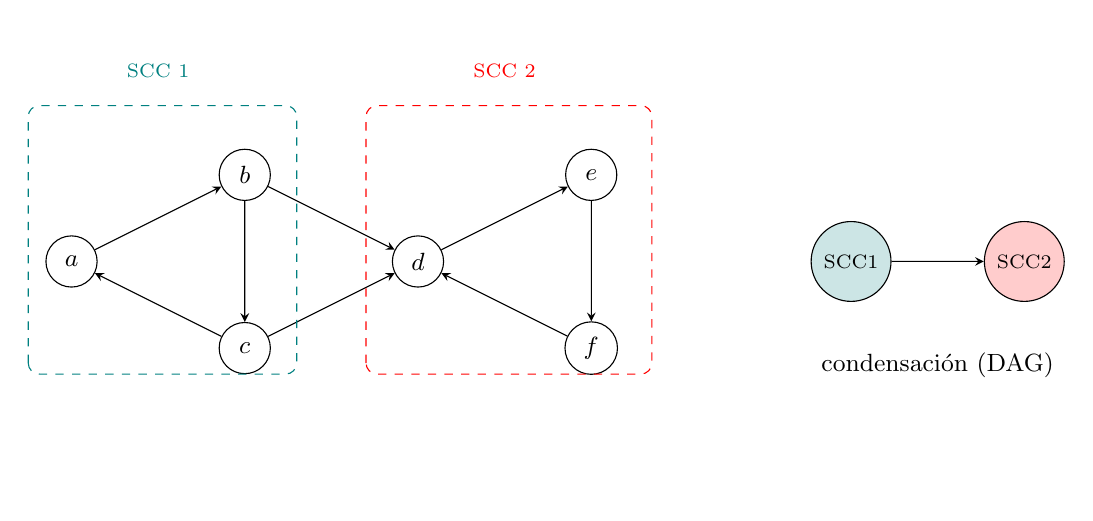
\begin{tikzpicture}[
  every node/.style={circle,draw,minimum size=0.65cm,font=\small},
  scale=1.1, ->, >=stealth
]
  \begin{scope}
    \node (a) at (0,2)   {$a$};
    \node (b) at (2,3)   {$b$};
    \node (c) at (2,1)   {$c$};
    \node (d) at (4,2)   {$d$};
    \node (e) at (6,3)   {$e$};
    \node (f) at (6,1)   {$f$};
    \draw (a)--(b); \draw (b)--(c); \draw (c)--(a);
    \draw (b)--(d); \draw (c)--(d);
    \draw (d)--(e); \draw (e)--(f); \draw (f)--(d);
    \draw[teal,dashed,rounded corners] (-0.5,0.7) rectangle (2.6,3.8);
    \draw[red,dashed,rounded corners] (3.4,0.7) rectangle (6.7,3.8);
    \node[draw=none,teal,font=\scriptsize] at (1.0,4.2) {SCC 1};
    \node[draw=none,red,font=\scriptsize] at (5.0,4.2) {SCC 2};
  \end{scope}
 
  \begin{scope}[xshift=9cm]
    \node[fill=teal!20,minimum size=0.9cm]  (s1) at (0,2) {\scriptsize SCC1};
    \node[fill=red!20,minimum size=0.9cm] (s2) at (2,2) {\scriptsize SCC2};
    \draw (s1)--(s2);
    \node[draw=none,font=\small] at (1,0.8) {condensación (DAG)};
  \end{scope}
\end{tikzpicture}
\end{figure}
La gráfica de condensación es útil porque permite aplicar programación
dinámica sobre el DAG para resolver preguntas sobre la gráfica original.
\section{2-SAT\adv}
\advnote{Requiere componentes fuertemente conexas (sección anterior). Puede omitirse en una primera lectura.}
Motivemos esta sección con este problema: \href{https://codeforces.com/problemset/problem/776/D}{The door problem}. Se nos dice que hay $n$ personas atrapadas en $n$ cuartos (una puerta por cuarto). Hay $m$ interrumptores; en general $m$ puede ser mayor, igual o menor que $n$, y no hay relación fija entre ambos. Activar o desactivar un interrumptor cambia el estado de las puertas que controla. Cada puerta es controlada por exactamente dos interrumptores. ¿Es posible operar los
interruptores para que todas las puertas queden desbloqueadas al mismo
tiempo?
\\\\
Para resolver este problema, usaremos componentes fuertemente conexas, en este momento puede que el lector no vea la relación entre las $SCC$ y el problema, pero esta sección buscará reducir el problema a $SCC$.
\\\\
Supongamos que tenemos $n$ variables booleanas, cada una puede ser verdadera ($V$) o falsa ($F$). Las \textbf{restricciones} exigen que ciertas condiciones se cumplan; cada una involucra dos literales (una variable o su negación) unidos por ``o''. Por ejemplo, con $n = 3$:
\begin{itemize}
    \item $(x_1 \lor x_2)$: al menos uno de $x_1$, $x_2$ debe ser verdadero.
    \item $(\neg x_1 \lor x_3)$: si $x_1$ es falso, entonces $x_3$ debe ser verdadero.
    \item $(\neg x_2 \lor \neg x_3)$: $x_2$ y $x_3$ no pueden ser verdaderos a la vez.
\end{itemize}
La asignación $x_1 = V,\; x_2 = F,\; x_3 = V$ satisface las tres. En general, la pregunta es: ¿existe una asignación de verdadero/falso a \emph{todas} las variables que cumpla \emph{todas} las restricciones?
\\\\
A diferencia del problema general de satisfacibilidad (que es
NP-completo), cuando cada restricción involucra \textbf{exactamente
dos variables} el problema se puede resolver en $O(V + E)$ usando SCCs.
Este caso especial se llama \textbf{2-SAT}.
\\\\
La observación fundamental que reduce este problema a $SCC$ es que toda disyunción de 2 literales $(a \lor b)$ es equivalente a dos implicaciones:
\[
\neg a \Rightarrow b \qquad \text{y} \qquad \neg b \Rightarrow a
\]
Si $a$ es falso, entonces $b$ debe ser verdadero (y viceversa).
\\\\
Esto permite construir una gráfica dirigida con $2n$ nodos ($x_i$ y $\neg x_i$ para cada variable) donde cada disyunción agrega dos aristas.
 
\begin{figure}[H]
\centering
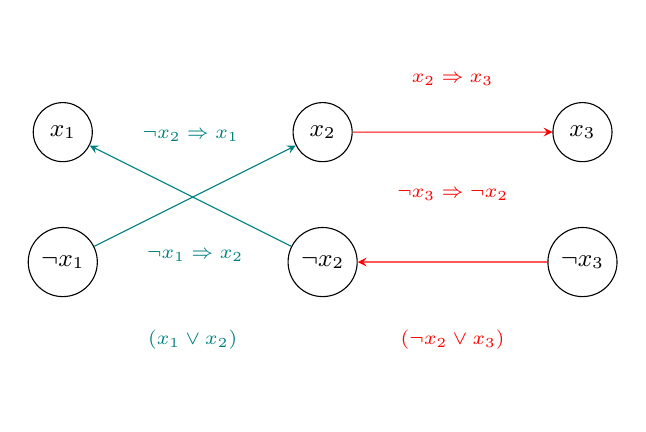
\begin{tikzpicture}[
  every node/.style={circle,draw,minimum size=0.75cm,font=\small},
  scale=1.1, ->, >=stealth
]
  \node (x1)  at (0,3)   {$x_1$};
  \node (nx1) at (0,1.5) {$\neg x_1$};
  \node (x2)  at (3,3)   {$x_2$};
  \node (nx2) at (3,1.5) {$\neg x_2$};
  \node (x3)  at (6,3)   {$x_3$};
  \node (nx3) at (6,1.5) {$\neg x_3$};
 
  \draw[teal] (nx1)--node[draw=none,below,font=\scriptsize]{$\neg x_1\Rightarrow x_2$}(x2);
  \draw[teal] (nx2)--node[draw=none,above,font=\scriptsize]{$\neg x_2\Rightarrow x_1$}(x1);
 
  \draw[red] (x2)--node[draw=none,above,font=\scriptsize]{$x_2\Rightarrow x_3$}(x3);
  \draw[red] (nx3)--node[draw=none,above,font=\scriptsize]{$\neg x_3\Rightarrow\neg x_2$}(nx2);
 
  \node[draw=none,font=\scriptsize,teal]  at (1.5,0.6) {$(x_1\lor x_2)$};
  \node[draw=none,font=\scriptsize,red] at (4.5,0.6) {$(\neg x_2\lor x_3)$};
\end{tikzpicture}
\end{figure}

Una fórmula 2-SAT es satisfacible si y solo si en el grafo de implicaciones ninguna variable $x_i$ está en la misma SCC que su negación $\neg x_i$. Si la fórmula es satisfacible, la asignación se obtiene directamente de los números de SCC que asigna Kosaraju:
 
\begin{itemize}
    \item $x_i = \text{verdadero}$ si $\text{comp}(x_i) > \text{comp}(\neg x_i)$
    \item $x_i = \text{falso}$ si $\text{comp}(x_i) < \text{comp}(\neg x_i)$
\end{itemize}
Kosaraju numera las SCCs de forma que si existe una implicación de la SCC $A$ hacia la SCC $B$, entonces $A$ recibe un número menor que $B$. La SCC con número mayor es la ``consecuencia'' de la cadena de implicaciones. Asignar verdadero a la variable cuya
SCC tiene número mayor garantiza que ninguna implicación se viola, siempre se va de falso hacia verdadero, nunca al revés.
\\\\
\\\\
En el problema de las puertas, cada puerta controlada por los interruptores $a$ y $b$ genera restricciones de exactamente esta forma.
\\\\Si la puerta está abierta, necesitamos que ambos interrumptores que la controlan se activen (sean verdaderos) o que ninguno lo haga (sean falsos). 
Esto se expresa con dos restricciones:
\begin{itemize}
    \item Si $x_a$ es verdadero, $x_b$ también debe serlo:
          $(\neg x_a \lor x_b)$
    \item Si $x_b$ es verdadero, $x_a$ también debe serlo:
          $(x_a \lor \neg x_b)$
\end{itemize}
Si está bloqueada, necesitamos que solamente uno de los interrumptores se active.
\begin{itemize}
    \item Si $x_a$ es verdadero, $x_b$ debe ser falso:
          $(\neg x_a \lor \neg x_b)$
    \item Si $x_a$ es falso, $x_b$ debe ser verdadero:
          $(x_a \lor x_b)$
\end{itemize}
Para resolver el problema entonces basta con construir la gráfica, correr Kosaraju y verificar que ningún $x_i$ esté en la misma SCC que $\neg x_i$.

\textbf{Ejercicio.} Implementar la solución del problema \href{https://codeforces.com/problemset/problem/776/D}{The door problem}.
 
\section{Puentes y puntos de articulación}
Para esta sección, pensemos el siguiente problema llamado \href{https://onlinejudge.org/external/3/315.pdfL}{Network}. En este problema, nos dicen que hay $n$ centrales de telefonía conectadas por cables bidireccionales de forma que desde cualquier central se puede llegar a otra no necesariamente de forma directa. En ocasiones, puede haber un apagón en alguna central por lo que deja de operar. Esto puede causar que otras centrales queden incomunicadas entre sí, en tal caso se dice son centrales críticas. Nos piden encontrar cuántas centrales son críticas.
\\\\
Nótese el siguiente ejemplo, si la central $4$ falla, las centrales
  $\{5,6\}$ quedan incomunicadas de $\{1,2,3\}$.
 
\begin{figure}[H]
\centering
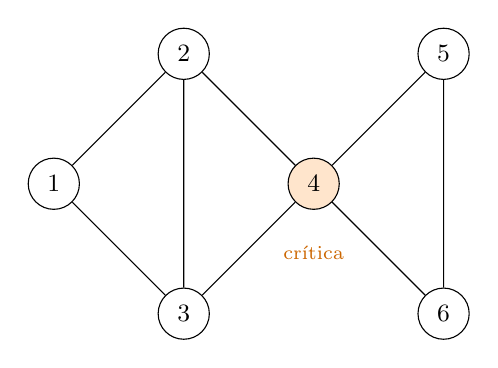
\begin{tikzpicture}[
  every node/.style={circle,draw,minimum size=0.65cm,font=\small},
  scale=1.1
]
  \node (1) at (0,1.5)  {1};
  \node (2) at (1.5,3)  {2};
  \node (3) at (1.5,0)  {3};
  \node[fill=orange!20] (4) at (3,1.5) {4};
  \node (5) at (4.5,3)  {5};
  \node (6) at (4.5,0)  {6};
 
  \draw (1)--(2) (2)--(3) (3)--(1);
  \draw (2)--(4) (3)--(4);
  \draw (4)--(5) (4)--(6) (5)--(6);
 
  \node[draw=none,font=\scriptsize,orange!80!black] at (3,0.7)
    {crítica};
\end{tikzpicture}
\end{figure}
  
\begin{definition}[Puente y punto de articulación]
En un grafo conexo $G$:
\begin{itemize}
    \item Una arista es un \textbf{puente} si al eliminarla el grafo
          se desconecta.
    \item Un vértice es un \textbf{punto de articulación} si al
          eliminarlo (junto con sus aristas incidentes) el grafo se
          desconecta.
\end{itemize}
\end{definition}

En la siguiente gráfica, la arista roja $d$-$e$ es un puente. Los vértices $d$ y $e$ porque al eliminarlos desconectan la gráfica.
\begin{figure}[H]
\centering
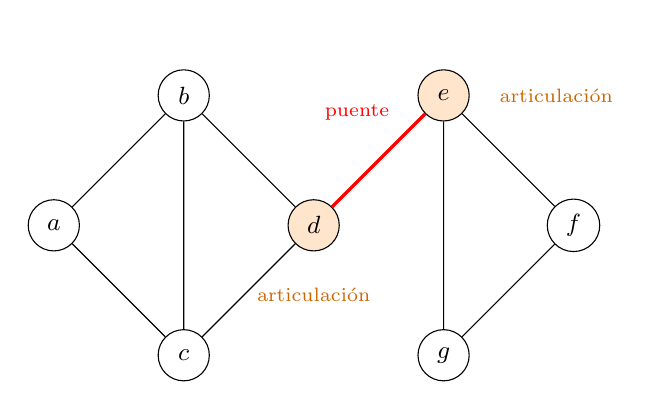
\begin{tikzpicture}[
  every node/.style={circle,draw,minimum size=0.65cm,font=\small},
  scale=1.1
]
  \node (a) at (0,1.5)  {$a$};
  \node (b) at (1.5,3)  {$b$};
  \node (c) at (1.5,0)  {$c$};
  \node[fill=orange!20] (d) at (3,1.5)  {$d$};
  \node[fill=orange!20] (e) at (4.5,3)  {$e$};
  \node (f) at (6,1.5)  {$f$};
  \node (g) at (4.5,0)  {$g$};
 
  \draw (a)--(b) (b)--(c) (c)--(a);
  \draw (b)--(d) (c)--(d);
  \draw[red,very thick] (d)--(e);
  \draw (e)--(f) (f)--(g) (g)--(e);
 
  \node[draw=none,font=\scriptsize,red]            at (3.5,2.8) {puente};
  \node[draw=none,font=\scriptsize,orange!80!black] at (3,0.7)  {articulación};
  \node[draw=none,font=\scriptsize,orange!80!black] at (5.8,3)  {articulación};
\end{tikzpicture}
\end{figure}
Regresando al problema de las centrales, notemos que el problema nos pide imprimir cuántos puntos de articulación tiene la gráfica dada. Podríamos intentar revisar cada vértice y ver si al quitarlo desconecta la gráfica con $BFS/DFS$ pero esto costaría $O((V+E)V)$ lo que nos daría $TLE$, necesitamos algo más eficiente.
\\\\
Al hacer DFS, el árbol de llamadas forma un árbol DFS. Las
aristas que no forman parte de este árbol conectan un nodo con algún \textbf{ancestro} suyo les llamaremos aristas hacia atrás.
\\\\
La idea para cosntruir un algoritmo más eficiente es ver que un nodo $U$ es punto de articulación si tiene algún hijo $V$ tal que
\textbf{ningún nodo del subárbol de $V$ puede llegar a un ancestro de
$U$ sin pasar por $U$}. Para revisar esto, asignamos a cada vértice
un tiempo de descubrimiento $\texttt{disc}[v]$ que corresponde al orden
en que el DFS lo visitó. Ahora definimos $\texttt{low}[v]$ como el menor $\texttt{disc}$ alcanzable desde el subárbol de $v$:
\[
\texttt{low}[v] = \min \begin{cases}
\texttt{disc}[v] \\
\texttt{disc}[u] & \text{para toda arista hacia atrás } (v,u) \\
\texttt{low}[w] & \text{para todo hijo } w \text{ de } v \text{ en el árbol DFS}
\end{cases}
\]
Intuitivamente, $\texttt{low}[v]$ mide qué tan ``arriba'' puede
escapar el subárbol de $v$ sin usar la arista que lo conecta a su padre. En la siguiente gráfica $v$ tiene $low=0$ porque tiene una arista hacia atrás que le permite llegar a $r$ que tiene $low=0$ sin pasar por su padre. De forma similar, $u$ hereda el $low=0$ de su hijo $u$.
 
\begin{figure}[H]
\centering
\begin{tikzpicture}[
  every node/.style={circle,draw,minimum size=0.65cm,font=\small},
  scale=1.1, ->, >=stealth
]
  \node (r) at (3,4)   {$r$};
  \node (u) at (3,2.5) {$u$};
  \node (v) at (3,1)   {$v$};
  \node (w) at (1.5,1) {$w$};
 
  \draw (r)--(u) (u)--(v) (u)--(w);
  \draw[teal,dashed,->] (v) to[bend right=50]
    node[draw=none,right,font=\scriptsize,teal]{arista hacia atrás}(r);
 
  \node[draw=none,left,font=\scriptsize] at (2.5,4.0)
    {$\texttt{disc}[r]=0,\ \texttt{low}[r]=0$};
  \node[draw=none,left,font=\scriptsize] at (2.5,2.5)
    {$\texttt{disc}[u]=1,\ \texttt{low}[r]=0$};
  \node[draw=none,right,font=\scriptsize] at (3.4,1)
    {$\texttt{disc}[v]=2,\ \texttt{low}[v]=0$};
  \node[draw=none,left,font=\scriptsize]  at (1.1,1)
    {$\texttt{disc}[w]=3,\ \texttt{low}[w]=3$};
\end{tikzpicture}
\end{figure}
Para que una arista $(uv)$  con $v$ hijo de $u$ n el DFS sea un puente, se debe cumplir que $\texttt{low}[v] > \texttt{disc}[u]$. Ya que eso significa que el subárbol de $v$ no puede alcanzar a $u$ sin pasar por la arista $(u,v)$. Dicho esto, es lógico que la condición para que un vértice $u$ sea punto de articulación sea:
\begin{itemize}
    \item Si $u$ es la raíz del DFS, es punto de articulación si tiene
          $\geq 2$ hijos en el árbol DFS.
    \item Si $u$ no es raíz, es punto de articulación si tiene algún hijo $v$ tal con $\texttt{low}[v] \geq \texttt{disc}[u]$.
\end{itemize}
Finalmente, la implementación nos quedaría:
\begin{lstlisting}[language=C++]
vector<int> adj[MAXN];
int disc[MAXN], low[MAXN], timer = 0;
bool visited[MAXN], art[MAXN];
vector<pair<int, int>> bridges;

void dfs(int u, int parent) {
    visited[u] = true;
    disc[u] = low[u] = timer++;
    int children = 0;

    for (int v : adj[u]) {
        if (!visited[v]) {
            children++;
            dfs(v, u);
            low[u] = min(low[u], low[v]);

            // Arista u-v es puente.
            if (low[v] > disc[u]) {
                bridges.push_back({u, v});
            }

            // u es articulacion (caso no raiz).
            if (parent != -1 && low[v] >= disc[u]) {
                art[u] = true;
            }
        } else if (v != parent) {
            // Arista hacia atras.
            low[u] = min(low[u], disc[v]);
        }
    }

    // u es articulacion (caso raiz).
    if (parent == -1 && children >= 2) {
        art[u] = true;
    }
}
\end{lstlisting}
\textbf{Ejercicio.} Implementar la solución completa de \href{https://onlinejudge.org/external/3/315.pdfL}{Network} usando
este algoritmo.
 
\section{Árboles}
 
Un \textbf{árbol} es un grafo conexo, es decir, todos sus vértices están conectados por un camino, sin ciclos. Esta definición es solo una de varias caracterizaciones equivalentes, todas igualmente válidas como definición y útiles en distintos contextos.
 
Para un grafo $G$ con $n$ vértices, las siguientes afirmaciones son equivalentes:
\begin{enumerate}
    \item $G$ es conexo y acíclico.
    \item $G$ es conexo y tiene exactamente $n-1$ aristas.
    \item Entre todo par de vértices existe exactamente un camino simple.
\end{enumerate}
 
La caracterización (3), camino único entre todo par, será importante porque convierte preguntas sobre caminos en preguntas sobre estructura del árbol. Es la base del LCA y de la mayoría de técnicas sobre árboles.
 
Para motivar este capítulo de árboles, véamos el problema \href{https://codeforces.com/contest/342/problem/E}{Xenia and Tree}, en este nos dan un árbol con n nodos. El nodo $1$ está pintado de rojo y los demás de azul. Nos darán queries de dos tipos:
\begin{itemize}
    \item[1.] Nos dan un numero $a$ que corresponde a un nodo azul y tenemos que pintarlo rojo.
    \item[2.] Nos dan un numero $b$ que corresponde a un nodo del arbol y tenemos que imprimir la distancia entre $b$ y el nodo rojo más cercano.
\end{itemize}
Nótese que calcular la distancia a cada uno de los nodos rojos cada que nos dan una querie no es eficiente y en este problema que nos pueden dar $10^5$ queries en un arbol de $10^5$ vértices, esta solución ingenua resultaría en $TLE$. Veremos algunas herramientas que nos ayudarían a resolver este problema.

\section{Centroide\adv}
\advnote{Requiere manejo cómodo de árboles (DFS, subtamaños). Puede omitirse en una primera lectura.}
 
El \textbf{centroide} de un árbol es un vértice $c$ tal que al eliminarlo, ninguna componente conexa resultante tiene más de $\lfloor n/2 \rfloor$ vértices. Todo árbol tiene uno o dos centroides. Si tiene dos, son adyacentes. En la siguiente figura el vértice amarillo es el centroide, nótese que entonces si se elimina las componentes conexas se quedan con un vértice.
 
\begin{figure}[H]
\centering
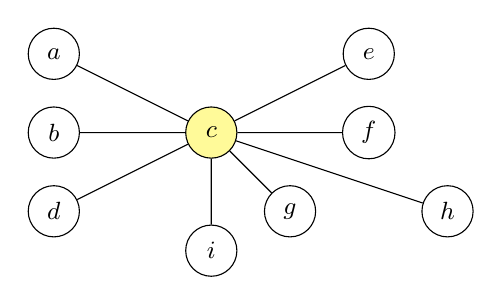
\begin{tikzpicture}[
  every node/.style={circle, draw, minimum size=0.65cm, font=\small},
  scale=1.0
]
  \node[fill=yellow!40] (c) at (3, 2) {$c$};
  \node (a) at (1, 3)   {$a$};
  \node (b) at (1, 2)   {$b$};
  \node (d) at (1, 1)   {$d$};
  \node (e) at (5, 3)   {$e$};
  \node (f) at (5, 2)   {$f$};
  \node (g) at (4, 1)   {$g$};
  \node (h) at (6, 1)   {$h$};
  \node (i) at (3, 0.5) {$i$};
 
  \draw (c)--(a) (c)--(b) (c)--(d) (c)--(e) (c)--(f) (c)--(g) (c)--(h) (c)--(i);
\end{tikzpicture}
\end{figure}
 
\subsubsection*{Descomposición por centroide}

Tomemos un árbol más grande que el anterior y tomemos su centroide $c$. Al eliminarlo, el árbol se divide en varias componentes, cada una de tamaño $\leq \lfloor n/2 \rfloor$. Nótese que entonces cualquier camino de un nodo $v$ en una componente a otro $u$ en otra componente, este pasa por $c$, entonces si quisieramos la distancia entre $u$ y $v$ podemos sumar la distancia entre $c$ y $v$ y la distancia entre $c$ y $u$.

\begin{figure}[H]
\centering
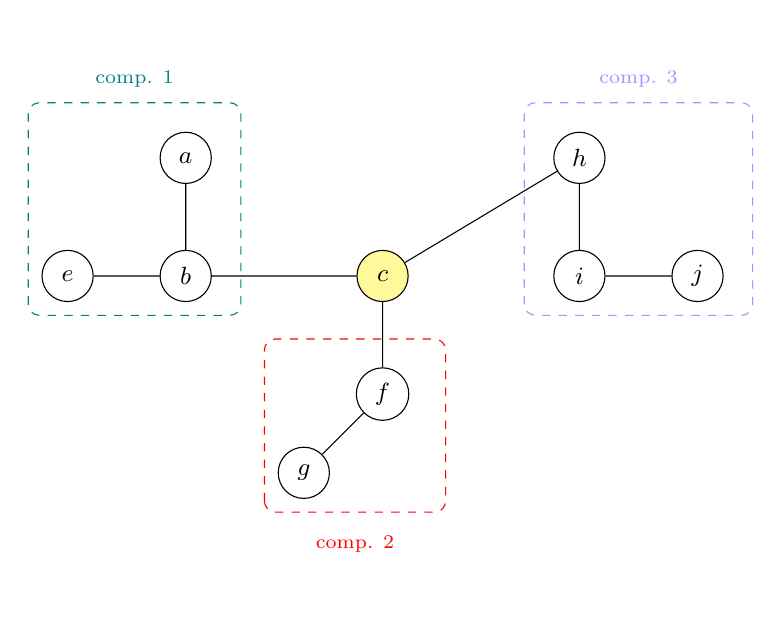
\begin{tikzpicture}[
  every node/.style={circle, draw, minimum size=0.65cm, font=\small},
  scale=1.0
]
  \node[fill=yellow!40] (c) at (4, 3) {$c$};
 
  \node (a) at (1.5, 4.5) {$a$};
  \node (b) at (1.5, 3.0) {$b$};
  \node (e) at (0.0, 3.0) {$e$};
 
  \node (f) at (4.0, 1.5) {$f$};
  \node (g) at (3.0, 0.5) {$g$};
 
  \node (h) at (6.5, 4.5) {$h$};
  \node (i) at (6.5, 3.0) {$i$};
  \node (j) at (8.0, 3.0) {$j$};
 
  \draw (b)--(a) (c)--(b) (c)--(f) (c)--(h);
 
  \draw (b)--(e) (f)--(g) (h)--(i) (i)--(j);
 
  \draw[dashed, teal, rounded corners] (-0.5,2.5) rectangle (2.2,5.2);
  \draw[dashed, red, rounded corners] (2.5,0.0) rectangle (4.8,2.2);
  \draw[dashed, blue!40, rounded corners] (5.8,2.5) rectangle (8.7,5.2);
 
  \node[draw=none, teal, font=\scriptsize] at (0.85, 5.5) {comp. 1};
  \node[draw=none, red, font=\scriptsize] at (3.65, -0.4) {comp. 2};
  \node[draw=none, blue!40, font=\scriptsize] at (7.25, 5.5) {comp. 3};
\end{tikzpicture}
\end{figure}
 La observación anterior solo resuelve caminos entre componentes distintas. Pero los nodos rojos también pueden estar en la misma componente que $v$. La solución es aplicar el mismo argumento recursivamente, cada componente tiene su propio centroide, y todo camino dentro de ella que no pasa por ese centroide, pasará por el centroide de alguna subcomponente más pequeña.

 Esto define el \textbf{árbol de centroide}: tomamos el centroide $c$ del árbol completo como raíz, recursamos en cada componente que queda al eliminarlo, y los centroides de esas componentes se vuelven hijos de $c$ en el árbol de centroide.
 
\begin{figure}[H]
\centering
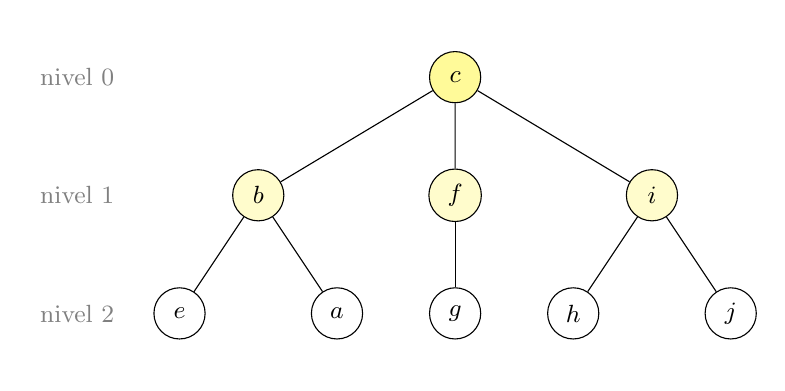
\begin{tikzpicture}[
  every node/.style={circle, draw, minimum size=0.65cm, font=\small},
  scale=1.0
]
  \node[fill=yellow!40] (c)  at (4.0, 4.0) {$c$};
  \node[fill=yellow!20] (c1) at (1.5, 2.5) {$b$};
  \node[fill=yellow!20] (c2) at (4.0, 2.5) {$f$};
  \node[fill=yellow!20] (c3) at (6.5, 2.5) {$i$};
  \node (e)  at (0.5, 1.0) {$e$};
  \node (a)  at (2.5, 1.0) {$a$};
  \node (g)  at (4.0, 1.0) {$g$};
  \node (h)  at (5.5, 1.0) {$h$};
  \node (j)  at (7.5, 1.0) {$j$};
 
  \draw (c)--(c1) (c)--(c2) (c)--(c3);
  \draw (c1)--(e) (c1)--(a);
  \draw (c2)--(g);
  \draw (c3)--(h) (c3)--(j);
 
  \node[draw=none, font=\small, gray] at (-0.8, 4.0) {nivel 0};
  \node[draw=none, font=\small, gray] at (-0.8, 2.5) {nivel 1};
  \node[draw=none, font=\small, gray] at (-0.8, 1.0) {nivel 2};
\end{tikzpicture}
\end{figure}

Notemos entonces que para cualquier par de nodos $u$ y $v$, existe un ancestro común en el árbol de centroide tal que el camino entre los nodos en el árbol original pasa por ese ancestro, el cual es el ancestro común de $u$ y $v$, por ejemplo, para $g$ y $e$ en el árbol anterior, este es $c$, es decir el primer ancestro que comparten. En caso de $e$ y $a$, es $b$.

%NOTA (buscar algun recuadro de color para estas cosas)
Una propiedad importante es que el árbol de centroide tiene profundidad $O(\log n)$, ya que cada vez que bajamos un nivel, el subárbol tiene tamaño $\leq \lfloor n/2 \rfloor$ (por la propiedad del centroide). Tras $k$ niveles el tamaño es $\leq n/2^k$. La recursión termina cuando el tamaño llega a 1, es decir a profundidad $\lceil \log_2 n \rceil$, esto es relevante para calcular la compleljidad del algortimo.

Volviendo al problema, con el árbol de centroide construido, mantenemos para cada nodo $c$:
\[
\texttt{minDist}[c] = \min_{u \text{ rojo}} \text{dist}(c,\, u)
\]
la distancia mínima desde $c$ a cualquier nodo rojo en el subárbol \emph{original} sobre el que $c$ fue centroide. Inicialmente $\texttt{minDist}[c] = \infty$ para todo $c$. Ahora, cada que recibamos una query del tipo $1$, en la que nos pidan pintar un vértice $v$ de rojo, para todo nodo $c$ ancestro de $v$ en el árbol de centroide, debemos actualizar:
\[
\texttt{minDist}[c] \leftarrow \min\, \!\bigl(\texttt{mindist}[c],\ \text{dist}(v, c)\bigr)
\]
Como hay $O(\log n)$ ancestros, esta operación cuesta $O(\log n)$ llamadas a \texttt{dist}.
 
\medskip
Para el segundo tipo de query notemos que para cualquier nodo rojo $u$, existe un ancestro $c$ de $v$ en el árbol de centroide tal que el camino de $v$ a $u$ pasa por $c$.
Entonces la respuesta es:
\[
\min_{c \text{ ancestro de } v \text{ en árbol de centroide}} \bigl(\text{dist}(v, c) + \texttt{minDist}[c]\bigr)
\]
De nuevo $O(\log n)$ llamadas a \texttt{dist}.
\\\\
Podría parecer que ya logramos optimizar la solución, sin embargo, estamos olvidando un detalle ¿cuánto cuesta calcular $\text{dist}(v, c)$?
\\\\
La forma más directa es hacer un BFS o DFS desde $c$ cada vez, pero eso cuesta $O(n)$ por llamada. Con $O(\log n)$ ancestros por query y $m$ queries, el costo total sería $O(mn \log n)$ que para $n = m = 10^5$ da $\sim 10^{11}$ operaciones. Demasiado lento.
\\\\
Necesitamos calcular $\text{dist}(u, v)$ en $O(\log n)$. Esto se logra con el \textbf{ancestro común más bajo} (LCA), que veremos en la siguiente sección.
\\\\
La implementación para construir el árbol de centroide queda:
\begin{lstlisting}[language=C++]
const int MAXN = 100005;

vector<int> g[MAXN];   // grafica original
int sz[MAXN];          // tamano del subarbol en la componente actual
bool removed[MAXN];    // true si el nodo ya fue usado como centroide
int cpar[MAXN];        // padre en el arbol de centroide (-1 para la raiz)

// Calcula el tamano del subarbol de u en la componente actual.
int calcSz(int u, int p) {
    sz[u] = 1;
    for (int v : g[u]) {
        if (v != p && !removed[v]) {
            sz[u] += calcSz(v, u);
        }
    }
    return sz[u];
}

// Encuentra el centroide de la componente que contiene a u.
int centroid(int u, int p, int treeSz) {
    for (int v : g[u]) {
        if (v != p && !removed[v] && sz[v] > treeSz / 2) {
            return centroid(v, u, treeSz);
        }
    }
    return u;
}

// Construye el arbol de centroide recursivamente.
// u: cualquier nodo de la componente actual.
// p: padre en el arbol de centroide (-1 para la raiz).
void build(int u, int p) {
    int total = calcSz(u, -1);
    int c = centroid(u, -1, total);

    cpar[c] = p;
    removed[c] = true;

    // Recursar en cada componente que queda al eliminar c.
    for (int v : g[c]) {
        if (!removed[v]) {
            build(v, c);
        }
    }
}
\end{lstlisting}
 El patrón estándar para cualquier problema que use descomposición por centroide es este problema, subir por los $O(\log n)$ ancestros en el árbol de centroide y agregar o consultar información en cada uno. Lo que varía entre problemas es qué información se guarda y cómo se combina.
\section{Ancestro común más bajo (LCA)\adv}
\advnote{Requiere árboles con raíz y, para la versión eficiente, preprocesamiento (binary lifting). Puede omitirse en una primera lectura.}
Dado un árbol con raíz, el \textbf{ancestro común más bajo} (LCA) de dos vértices $u$ y $v$ es el vértice más abajo que es ancestro de ambos.
\begin{figure}[H]
\centering
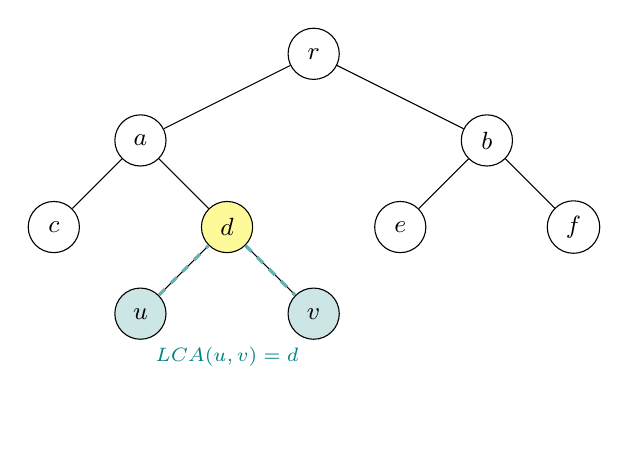
\begin{tikzpicture}[
  every node/.style={circle, draw, minimum size=0.65cm, font=\small},
  scale=1.1
]
  \node (r) at (4, 4)   {$r$};
  \node (a) at (2, 3)   {$a$};
  \node (b) at (6, 3)   {$b$};
  \node (c) at (1, 2)   {$c$};
  \node[fill=yellow!40] (d) at (3, 2) {$d$};
  \node (e) at (5, 2)   {$e$};
  \node (f) at (7, 2)   {$f$};
  \node[fill=teal!20] (u) at (2, 1)   {$u$};
  \node[fill=teal!20] (v) at (4, 1)   {$v$};
 
  \draw (r)--(a) (r)--(b) (a)--(c) (a)--(d) (b)--(e) (b)--(f) (d)--(u) (d)--(v);
 
  \draw[teal!60, very thick, dashed] (u)--(d)--(v);
  \node[draw=none, font=\scriptsize, teal] at (3, 0.5) {$\text{LCA}(u,v) = d$};
\end{tikzpicture}
\end{figure}
La solución más directa que podríamos pensar es ver qué nodo está más bajo o profundo y llevarlo al mismo nivel que el otro subiendo de a un paso, luego subir ambos juntos hasta que coincidan. Por ejemplo para $c$ y $u$ en la figura de arriba, primero subiríamos $u$ a su ancestro $d$ y ya que ambos $d$ y $c$ estpan en el mismo nivel, los subiriamos a su ancestro $a$ que como coincide, diríamos que este es su $LCA$.
\\\\
Imaginemos que tenemos un árbol en forma de cadena ($1 - 2 - 3 - \cdots - n$), calcular $\text{LCA}(1, n)$ cuesta $O(n)$ pasos. Con $m$ queries, el costo total es $O(mn)$, lo que nos deja con el mismo problema que teníamos antes, necesitamos algo más eficiente. En lugar de subir de $1$ en $1$, ¿podríamos subir de a $2^k$ niveles de una vez?
\\\\
 Para subir $d$ niveles desde un nodo $v$, podemos descomponer $d$ en potencias de 2 (como en la representación binaria) y dar saltos de tamaño $1, 2, 4, 8, \ldots$ según corresponda. Si $d = 13 = 8 + 4 + 1$, damos un salto de 8, luego uno de 4, luego uno de 1, tres saltos en lugar de 13.
\\\\
Entonces necesitamos precalcular, para cada nodo $v$ y cada $k$:
\[
\texttt{up}[v][k] = \text{ancestro de } v \text{ a distancia } 2^k
\]
La forma de calcular esto será con una recurrencia, el ancestro a distancia $2^k$ es el ancestro a distancia $2^{k-1}$ del ancestro a distancia $2^{k-1}$:
\[
\texttt{up}[v][0] = \text{padre}(v), \qquad \texttt{up}[v][k] = \texttt{up}[\texttt{up}[v][k-1]][k-1]
\]
 
Como estamos subiendo en potencias de $2$, $\lfloor \log_2 n \rfloor + 1$ niveles basta para cubrir cualquier distancia hasta $n$. En la siguiente imagen, vemos como para el arbol que es una cadena que mencionamos antes, esta forma de encontrar el ancestro sí resulta eficiente. Para el nodo $v$, los ancestros a distancia $2^0=1$, $2^1=2$ y $2^2=4$ se precalculan. Para subir 5 niveles, basta un salto de 4 y un salto de 1, solo 2 operaciones.
 
\begin{figure}[H]
\centering
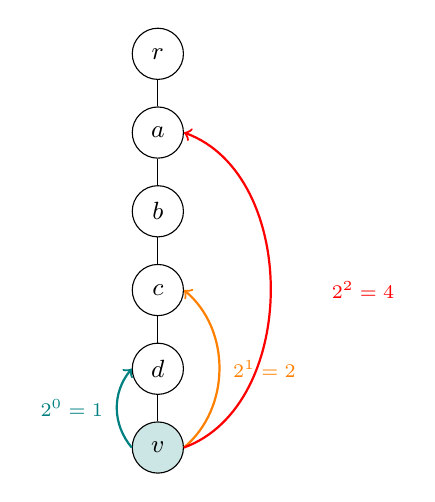
\begin{tikzpicture}[
  every node/.style={circle, draw, minimum size=0.65cm, font=\small},
  scale=1.0
]
  \node (r)  at (4.0, 5.0) {$r$};
  \node (a)  at (4.0, 4.0) {$a$};
  \node (b)  at (4.0, 3.0) {$b$};
  \node (c)  at (4.0, 2.0) {$c$};
  \node (d)  at (4.0, 1.0) {$d$};
  \node[fill=teal!20] (v)  at (4.0, 0.0) {$v$};
 
  \draw (r)--(a)--(b)--(c)--(d)--(v);
 
  \draw[teal, thick, ->] (v.west) to[bend left=40]
    node[draw=none, left, font=\scriptsize] {$2^0=1$} (d.west);
 
  \draw[orange, thick, ->] (v.east) to[bend right=50]
    node[draw=none, right, font=\scriptsize] {$2^1=2$} (c.east);
 
  \draw[red, thick, ->] (v.east) to[bend right=70]
    node[draw=none, right=0.6cm, font=\scriptsize] {$2^2=4$} (a.east);
\end{tikzpicture}
\end{figure}

Lo que haremos entonces para calcular el $LCA$  de dos nodos $u$ y $v$ será primero igualar sus profundidades. Si $\text{prof}(u) > \text{prof}(v)$, necesitamos subir $u$ exactamente $d = \text{prof}(u) - \text{prof}(v)$ niveles. Descomponemos $d$ en binario y usamos los saltos correspondientes.
\\\\
Una vez que coinciden, revisamos si $u = v$, ai se cumple, ese es el LCA. De lo contrario, subimos ambos nodos simultáneamente, usando el salto más grande posible tal que $\texttt{up}[u][k] \neq \texttt{up}[v][k]$ (es decir, que no hayan convergido todavía). Después de este proceso, $u$ y $v$ son hijos del LCA.

\begin{lstlisting}[language=C++]
const int LOG = 17;
int up[MAXN][LOG];  // up[v][k] = ancestro de v a distancia 2^k
int prof[MAXN];

// Precalcula ancestros con DFS desde la raiz.
void dfs(int v, int p, int d) {
    up[v][0] = p;
    prof[v] = d;

    for (int k = 1; k < LOG; k++) {
        up[v][k] = up[up[v][k - 1]][k - 1];
    }

    for (int u : g[v]) {
        if (u != p) {
            dfs(u, v, d + 1);
        }
    }
}

int lca(int u, int v) {
    // Igualar profundidades.
    if (prof[u] < prof[v]) {
        swap(u, v);
    }
    int diff = prof[u] - prof[v];
    for (int k = 0; k < LOG; k++) {
        if ((diff >> k) & 1) {
            u = up[u][k];
        }
    }

    if (u == v) {
        return u;
    }

    // Subir ambos nodos juntos hasta quedar justo debajo del LCA.
    for (int k = LOG - 1; k >= 0; k--) {
        if (up[u][k] != up[v][k]) {
            u = up[u][k];
            v = up[v][k];
        }
    }

    return up[u][0];
}
\end{lstlisting}

Notemos que para calcular la distancia entre dos nodos $u$ y $v$, el camino de $u$ a $v$ sube desde $u$ hasta el LCA $d$ y luego baja hasta $v$. La distancia total es la suma de los dos tramos, que se simplifica a $\text{prof}(u)+\text{prof}(v)-2\cdot\text{prof}(\text{LCA})$.
\begin{figure}[H]
\centering
\begin{tikzpicture}[
  every node/.style={circle, draw, minimum size=0.7cm, font=\small},
  scale=1.15
]
 
\node (r) at (4.0, 5.0) {$r$};
\node (a) at (2.0, 4.0) {$a$};
\node (b) at (6.0, 4.0) {$b$};
\node (c) at (1.0, 3.0) {$c$};
\node[fill=yellow!40] (d) at (3.0, 3.0) {$d$};
\node (e) at (5.0, 3.0) {$e$};
\node (f) at (7.0, 3.0) {$f$};
\node[fill=teal!20] (u) at (2.0, 2.0) {$u$};
\node[fill=teal!20] (v) at (4.0, 2.0) {$v$};
 
\draw[gray!60] (r)--(a) (r)--(b);
\draw[gray!60] (a)--(c) (a)--(d);
\draw[gray!60] (b)--(e) (b)--(f);
 
\draw[teal, very thick] (u)--(d)--(v);
 
\draw[dashed, gray!50] (3.0, 4.85) -- (3.0, 3.35);
\draw[gray!50] (3.0, 4.85) -- (3.2, 4.85);
\draw[gray!50] (3.0, 3.35) -- (3.2, 3.35);
\node[draw=none, right, font=\scriptsize, text=gray] at (3.2, 4.1) {$\text{prof}(d) = 2$};
 
\draw[teal!60, dashed] (0.5, 4.85) -- (0.5, 2.35);
\draw[teal!60] (0.5, 4.85) -- (0.7, 4.85);
\draw[teal!60] (0.5, 2.35) -- (0.7, 2.35);
\node[draw=none, left, font=\scriptsize, text=teal!80!black] at (0.5, 3.6)
  {$\text{prof}(u) = 3$};
 
\node[draw=none, below right, font=\scriptsize, text=orange!70!black] at (2.5, 4.1)
  {\textbf{LCA}$(u,v)$};
 
\node[draw=none, right, font=\small] at (7.8, 3.5) {
  $\begin{aligned}
    \text{dist}(u,v)
      &= \underbrace{\text{prof}(u) - \text{prof}(d)}_{\text{subida}} 
       + \underbrace{\text{prof}(v) - \text{prof}(d)}_{\text{bajada}}\\[4pt]
      &= \text{prof}(u) + \text{prof}(v) - 2\cdot\text{prof}(d)\\[4pt]
      &= 3 + 3 - 2\cdot 2 = 2\ 
  \end{aligned}$
};
\end{tikzpicture}
\end{figure}

Finalmente, volviendo al problema, con \texttt{dist(u, v)} implementado en $O(\log n)$, la solución completa consiste en:
 
\begin{enumerate}
    \item Preprocesar LCA con DFS. $O(n \log n)$.
    \item Construir el árbol de centroide. $O(n \log n)$.
    \item Para cada query de tipo 1 (pintar $v$), subir $O(\log n)$ ancestros en el árbol de centroide, calcular \texttt{dist} en $O(\log n)$ en cada uno. $O(\log^2 n)$.
    \item Para cada query de tipo 2 (distancia mínima desde $v$), igual que el tipo 1, subir $O(\log n)$ ancestros en el árbol de centroide calculando \texttt{dist} en $O(\log n)$ en cada uno. $O(\log^2 n)$.
\end{enumerate}
 
Nótese que la complejidad es $O(n \log n + m \log^2 n)$, que para $n = m = 10^5$ da $\sim 10^7$ operaciones, lo que sí es eficiente.
 
\textbf{Ejercicio.} Implementar la solución completa del problema \href{https://codeforces.com/contest/342/problem/E}{Xenia and Tree (Codeforces 342E)} usando lo visto en esta sección.
 
\section{Flujo máximo\adv}
\advnote{Tema avanzado de gráficas: incluye Ford--Fulkerson, Dinic, matching y los teoremas de König y Hall. Puede omitirse en una primera lectura.}
Imagina que tienes una red de servidores conectados por cables. Cada cable tiene un ancho de banda máximo (en MB/s). Quieres descargar un archivo de un servidor $s$ a un servidor $t$ lo más rápido posible. Puedes dividir la descarga en varias rutas que pasen información simultáneamente, pero ningún cable puede superar su capacidad. ¿Cuántos MB/s puedes transferir en total?
 
\begin{figure}[H]
\centering
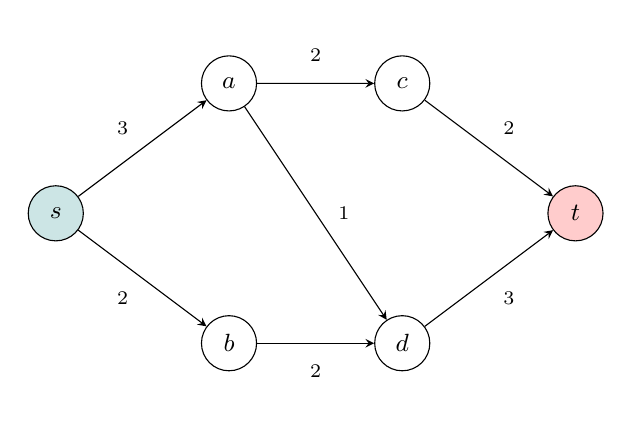
\begin{tikzpicture}[
  every node/.style={circle, draw, minimum size=0.7cm, font=\small},
  scale=1.1, ->, >=stealth
]
  \node[fill=teal!20]  (s) at (0, 1.5) {$s$};
  \node (a) at (2, 3)   {$a$};
  \node (b) at (2, 0)   {$b$};
  \node (c) at (4, 3)   {$c$};
  \node (d) at (4, 0)   {$d$};
  \node[fill=red!20] (t) at (6, 1.5) {$t$};
 
  \draw (s) -- node[draw=none,above left,font=\scriptsize]  {3} (a);
  \draw (s) -- node[draw=none,below left,font=\scriptsize]  {2} (b);
  \draw (a) -- node[draw=none,above,font=\scriptsize]       {2} (c);
  \draw (a) -- node[draw=none,right,font=\scriptsize]       {1} (d);
  \draw (b) -- node[draw=none,below,font=\scriptsize]       {2} (d);
  \draw (c) -- node[draw=none,above right,font=\scriptsize] {2} (t);
  \draw (d) -- node[draw=none,below right,font=\scriptsize] {3} (t);
\end{tikzpicture}
\end{figure}
 
Lo que buscamos se llama el \textbf{flujo máximo} de $s$ a $t$; sin embargo antes del algoritmo, veremos algunas definiciones que nos serán de utilidad.
\begin{definition}[Red de flujo]
Una \textbf{red de flujo} es una gráfica dirigida $G = (V, E)$ con:
\begin{itemize}
    \item Una función de \textbf{capacidad} $c: E \to \mathbb{R}_{\geq 0}$
          (el ancho de banda de cada cable).
    \item Una \textbf{fuente} $s$ (servidor de origen) y un
          \textbf{sumidero} $t$ (servidor de destino).
\end{itemize}
Un \textbf{flujo factible} es una función $f: E \to \mathbb{R}_{\geq 0}$
que satisface:
\begin{itemize}
    \item \textbf{Capacidad}: $0 \leq f(u,v) \leq c(u,v)$ para toda
          arista, no se puede superar el ancho de banda del cable.
    \item \textbf{Conservación}: para todo $v \neq s, t$:
          \[
          \sum_{u} f(u,v) = \sum_{w} f(v,w)
          \]
          lo que llega a un servidor intermedio también sale de él.
\end{itemize}
El \textbf{valor del flujo} es $|f| = \sum_v f(s,v)$: cuántos MB/s
salen de $s$ en total.
\end{definition}
 
\begin{definition}[Gráfica residual]
Dado un flujo $f$, la \textbf{gráfica residual} $G_f$ indica cuánta
capacidad queda disponible para ajustar el flujo. Por cada cable
$(u,v)$ se construyen las siguientes aristas dirigidas si la capacidad residual corresponndiente es mayor a $0$:
\begin{itemize}
    \item $(u,v)$ con capacidad residual $c(u,v) - f(u,v)$, cuánto más puedo enviar por este cable.
    \item $(v,u)$ con capacidad residual $f(u,v)$, cuánto flujo puedo ``cancelar'', es decir redirigir a otra ruta.
\end{itemize}
\end{definition}
 
La arista hacia atrás es la idea clave que permite corregir decisiones
anteriores. Si envié 2 MB/s por el cable $(u,v)$ y encuentro una ruta
mejor que pasa por $(v,u)$, puedo ``devolver'' hasta 2 MB/s de ese
cable y redirigirlos.

\subsection{Ford-Fulkerson}
 
La idea de este algoritmo es tomar la gráfica residual y mientras exista una ruta de $s$ a $t$ con capacidad disponible, enviar flujo por ella. En la siguiente red, todas las capacidades son $1$ y el flujo máximo es $2$ (ruta $s\to u\to t$ y ruta $s\to v\to t$ simultáneamente).
 
\begin{figure}[H]
\centering
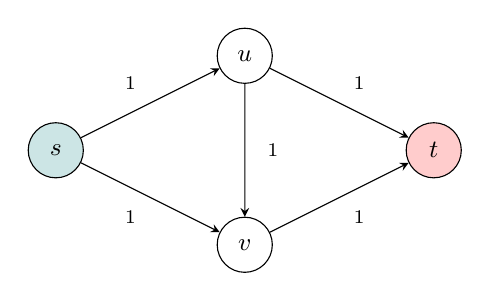
\begin{tikzpicture}[
  every node/.style={circle,draw,minimum size=0.7cm,font=\small},
  scale=1.2, ->, >=stealth
]
  \node[fill=teal!20]  (s) at (0,1)  {$s$};
  \node (u) at (2,2)   {$u$};
  \node (v) at (2,0)   {$v$};
  \node[fill=red!20] (t) at (4,1)  {$t$};
 
  \draw (s)--node[draw=none,above left,font=\scriptsize]{1}(u);
  \draw (s)--node[draw=none,below left,font=\scriptsize]{1}(v);
  \draw (u)--node[draw=none,right,font=\scriptsize]{1}(v);
  \draw (u)--node[draw=none,above right,font=\scriptsize]{1}(t);
  \draw (v)--node[draw=none,below right,font=\scriptsize]{1}(t);
\end{tikzpicture}
\end{figure}
 
Lo primero que haríamos sería buscar cualquier ruta de $s$ a $t$ con capacidad disponible. Encontramos $s \to u \to v \to t$ (capacidad 1 en cada cable). Enviamos 1 MB/s por esta ruta.
 
\begin{figure}[H]
\centering
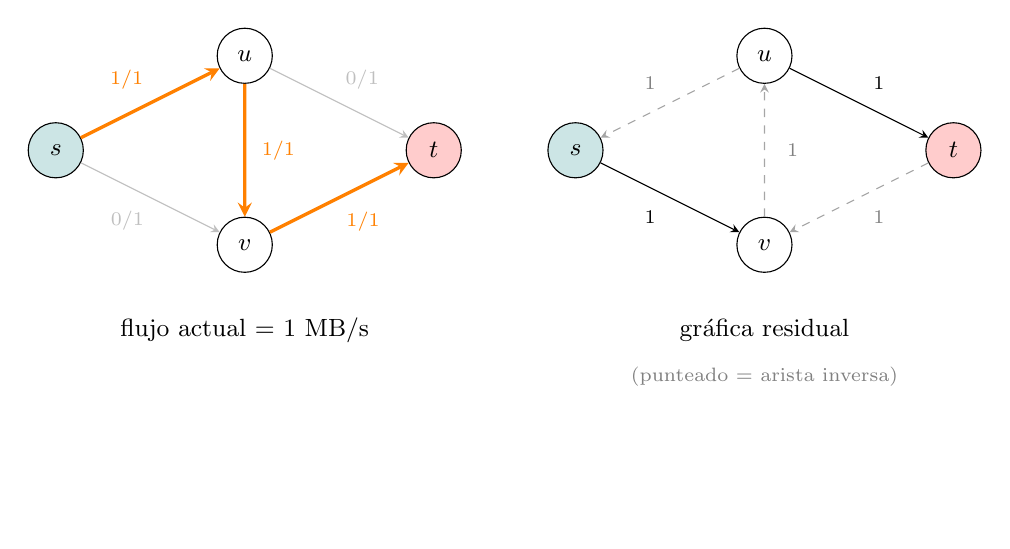
\begin{tikzpicture}[
  every node/.style={circle,draw,minimum size=0.7cm,font=\small},
  scale=1.2, ->, >=stealth
]
  \node[fill=teal!20]  (s) at (0,1)  {$s$};
  \node (u) at (2,2)   {$u$};
  \node (v) at (2,0)   {$v$};
  \node[fill=red!20] (t) at (4,1)  {$t$};
 
  \draw[orange,very thick] (s)--node[draw=none,above left,font=\scriptsize]{1/1}(u);
  \draw[gray!50]           (s)--node[draw=none,below left,font=\scriptsize]{0/1}(v);
  \draw[orange,very thick] (u)--node[draw=none,right,font=\scriptsize]{1/1}(v);
  \draw[gray!50]           (u)--node[draw=none,above right,font=\scriptsize]{0/1}(t);
  \draw[orange,very thick] (v)--node[draw=none,below right,font=\scriptsize]{1/1}(t);
 
  \node[draw=none,font=\small] at (2,-0.9)
    {flujo actual = 1 MB/s};
 
  \begin{scope}[xshift=5.5cm]
    \node[fill=teal!20]  (s2) at (0,1) {$s$};
    \node (u2) at (2,2)  {$u$};
    \node (v2) at (2,0)  {$v$};
    \node[fill=red!20] (t2) at (4,1) {$t$};
 
    \draw[gray!70,dashed] (u2)--node[draw=none,above left,font=\scriptsize,gray]{1}(s2);
    \draw (s2)--node[draw=none,below left,font=\scriptsize]{1}(v2);
    \draw[gray!70,dashed] (v2)--node[draw=none,right,font=\scriptsize,gray]{1}(u2);
    \draw (u2)--node[draw=none,above right,font=\scriptsize]{1}(t2);
    \draw[gray!70,dashed] (t2)--node[draw=none,below right,font=\scriptsize,gray]{1}(v2);
 
    \node[draw=none,font=\small] at (2,-0.9) {gráfica residual};
    \node[draw=none,font=\scriptsize,gray] at (2,-1.4) {(punteado = arista inversa)};
  \end{scope}
\end{tikzpicture}
\end{figure}
Mirando el grafo residual, buscamos otra ruta de $s$ a $t$. Vemos que $s\to v\to t$ no funciona porque $v\to t$ está saturado (capacidad
residual 0).
\\\\
Pero notemos que la ruta $s \to v \to u \to t$ usa la \textbf{arista inversa} $v\to u$ y así ``cancela'' 1 MB/s que íbamos enviando de $u$ a $v$, y lo redirige directamente de $u$ a $t$.
 
\begin{figure}[H]
\centering
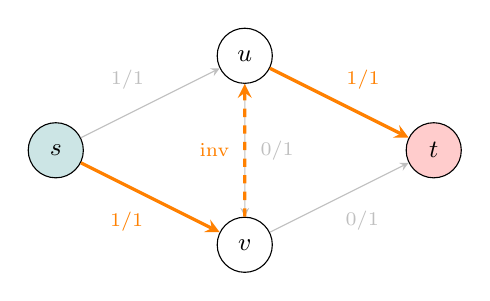
\begin{tikzpicture}[
  every node/.style={circle,draw,minimum size=0.7cm,font=\small},
  scale=1.2, ->, >=stealth
]
  \node[fill=teal!20]  (s) at (0,1) {$s$};
  \node (u) at (2,2)  {$u$};
  \node (v) at (2,0)  {$v$};
  \node[fill=red!20] (t) at (4,1) {$t$};
 
  \draw[gray!50]           (s)--node[draw=none,above left,font=\scriptsize]{1/1}(u);
  \draw[orange,very thick] (s)--node[draw=none,below left,font=\scriptsize]{1/1}(v);
  \draw[gray!50]           (u)--node[draw=none,right,font=\scriptsize]{0/1}(v);
  \draw[orange,very thick] (u)--node[draw=none,above right,font=\scriptsize]{1/1}(t);
  \draw[gray!50]           (v)--node[draw=none,below right,font=\scriptsize]{0/1}(t);
 
  \draw[orange,very thick,dashed] (v)--node[draw=none,left,font=\scriptsize,orange]{inv}(u);
\end{tikzpicture}
\end{figure}
 Enviamos 1 MB/s por esta ruta y actualizamos:
\begin{center}
\begin{tabular}{lccc}
\toprule
Cable & Flujo antes & Cambio & Flujo después \\
\midrule
$s\to v$ & 0 & $+1$ & 1 \\
$v\to u$ (inversa) & — & cancela $u\to v$ & — \\
$u\to v$ & 1 & $-1$ & \textbf{0} \\
$u\to t$ & 0 & $+1$ & 1 \\
\midrule
$s\to u$ & 1 & sin cambio & 1 \\
$v\to t$ & 1 & sin cambio & 1 \\
\bottomrule
\end{tabular}
\end{center}
Nótese que entonces nos deja con el siguiente flujo en la red original:
\begin{figure}[H]
\centering
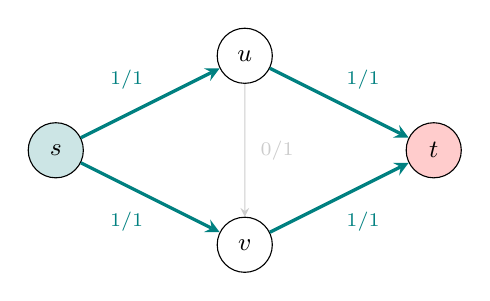
\begin{tikzpicture}[
  every node/.style={circle,draw,minimum size=0.7cm,font=\small},
  scale=1.2, ->, >=stealth
]
  \node[fill=teal!20]  (s) at (0,1) {$s$};
  \node (u) at (2,2)  {$u$};
  \node (v) at (2,0)  {$v$};
  \node[fill=red!20] (t) at (4,1) {$t$};
 
  \draw[teal,very thick] (s)--node[draw=none,above left,font=\scriptsize]{1/1}(u);
  \draw[teal,very thick] (s)--node[draw=none,below left,font=\scriptsize]{1/1}(v);
  \draw[gray!40]         (u)--node[draw=none,right,font=\scriptsize]{0/1}(v);
  \draw[teal,very thick] (u)--node[draw=none,above right,font=\scriptsize]{1/1}(t);
  \draw[teal,very thick] (v)--node[draw=none,below right,font=\scriptsize]{1/1}(t);
\end{tikzpicture}
\end{figure}
No hay más rutas disponibles en la gráfica residual, es aquí cuándo el algoritmo termina con flujo máximo = \textbf{2 MB/s}.
\\\\
Notemos que con capacidades enteras, cada iteración aumenta el
flujo en al menos 1, dando $O(|f^*| \cdot E)$ iteraciones donde $|f^*|$
es el flujo máximo. Si las capacidades son grandes esto es bastante lento, es por esto que veremos otro algoritmo que lo resuelve más rápido.
\subsection{Dinic} 
Dinic resuelve el problema de la cantidad de iteraciones eligiendo
sistemáticamente los caminos \textbf{más cortos} primero y saturando
\textbf{todos} los de esa longitud antes de pasar a los más largos. Veámos con el siguiente ejemplo cómo funciona:
 \\\\Lo primero que haremos será correr un $BFS$ desde $s$ para calcular las distancias de $s$ a los nodos y asignar niveles que representaremos con $\ell$. Véase que $t$ es alcanzable a distancia 3 (por $c\to t$) y también a distancia 4 (por $e\to t$),entonces $\ell(t)=3$. Para que una arista $(u,v)$ entre en la gráfica por niveles debe cumplir una regla: $\ell(v) = \ell(u)+1$. La arista $e\to t$ no cumple, pues ($\ell(t)=3 \neq \ell(e)+1=4$) por lo que se ignora.
 
\begin{figure}[H]
\centering
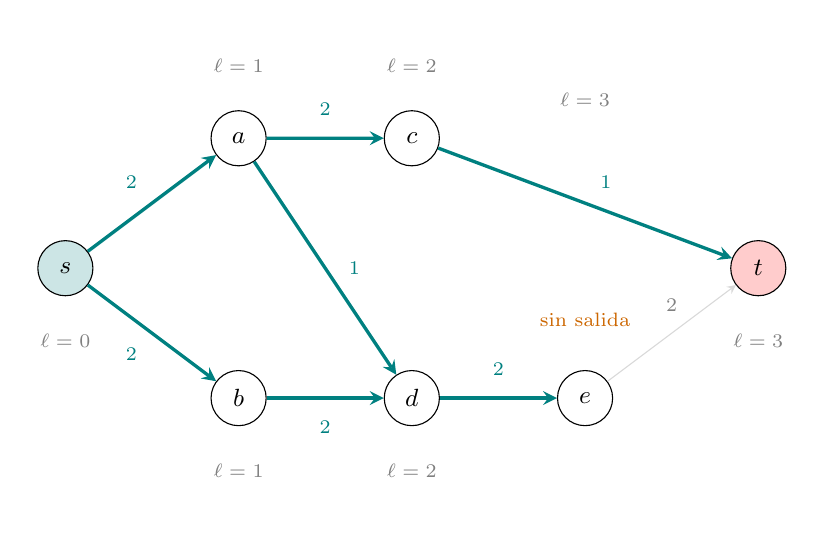
\begin{tikzpicture}[
  every node/.style={circle,draw,minimum size=0.7cm,font=\small},
  scale=1.1, ->, >=stealth
]
  \node[fill=teal!20]  (s) at (0,1.5)  {$s$};
  \node (a) at (2,3)    {$a$};
  \node (b) at (2,0)    {$b$};
  \node (c) at (4,3)    {$c$};
  \node (d) at (4,0)    {$d$};
  \node (e) at (6,0)  {$e$};
  \node[fill=red!20] (t) at (8,1.5)  {$t$};
 
  \draw[teal,very thick] (s)--node[draw=none,above left,font=\scriptsize]{2}(a);
  \draw[teal,very thick] (s)--node[draw=none,below left,font=\scriptsize]{2}(b);
  \draw[teal,very thick] (a)--node[draw=none,above,font=\scriptsize]{2}(c);
  \draw[teal,very thick] (a)--node[draw=none,right,font=\scriptsize]{1}(d);
  \draw[teal,very thick] (b)--node[draw=none,below,font=\scriptsize]{2}(d);
  \draw[teal,very thick] (c)--node[draw=none,above right,font=\scriptsize]{1}(t);
  \draw[teal,very thick] (d)--node[draw=none,above,font=\scriptsize]{2}(e);
  \draw[gray!30] (e)--node[draw=none,above,font=\scriptsize,gray]{2}(t);

  \node[draw=none,font=\scriptsize,orange!80!black] at (6,0.9) {sin salida};
 
  \node[draw=none,below,font=\scriptsize,gray] at (0,1.1)   {$\ell=0$};
  \node[draw=none,above,font=\scriptsize,gray] at (2,3.4)   {$\ell=1$};
  \node[draw=none,below,font=\scriptsize,gray] at (2,-0.4)  {$\ell=1$};
  \node[draw=none,above,font=\scriptsize,gray] at (4,3.4)   {$\ell=2$};
  \node[draw=none,below,font=\scriptsize,gray] at (4,-0.4)  {$\ell=2$};
  \node[draw=none,above,font=\scriptsize,gray] at (6,3)   {$\ell=3$};
  \node[draw=none,below,font=\scriptsize,gray] at (8,1.1)   {$\ell=3$};
\end{tikzpicture}
\end{figure}
Notemos que el único camino disponible es $s\to a\to c\to t$, el flujo que salga de este será entonces $\min(2,2,1) = 1$. El cable $c\to t$ queda saturado.
\\\\
Ahora, el BFS en la gráfica residual ya no puede llegar a $t$ por $c\to t$
(saturado). Ahora la ruta más corta a $t$ pasa por $e$ y tiene longitud 4:
 
\begin{figure}[H]
\centering
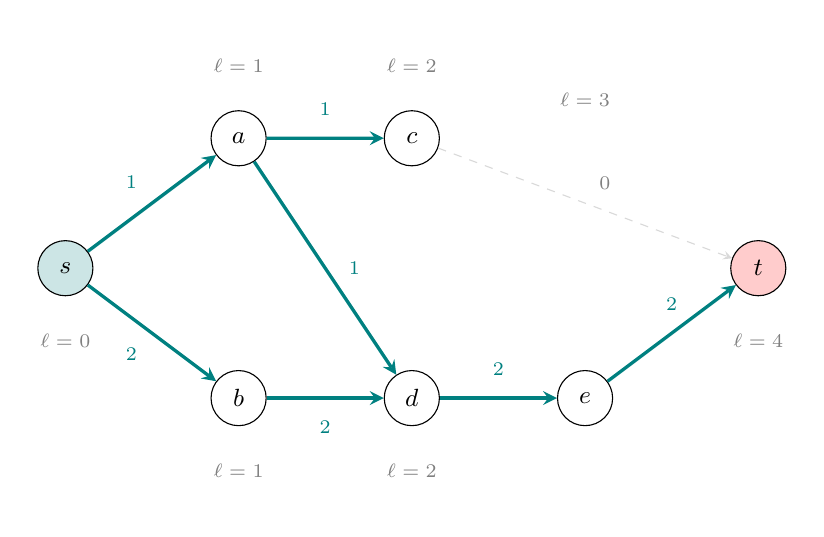
\begin{tikzpicture}[
  every node/.style={circle,draw,minimum size=0.7cm,font=\small},
  scale=1.1, ->, >=stealth
]
  \node[fill=teal!20]  (s) at (0,1.5)  {$s$};
  \node (a) at (2,3)    {$a$};
  \node (b) at (2,0)    {$b$};
  \node (c) at (4,3)    {$c$};
  \node (d) at (4,0)    {$d$};
  \node (e) at (6,0)  {$e$};
  \node[fill=red!20] (t) at (8,1.5)  {$t$};
 
  \draw[teal,very thick] (s)--node[draw=none,above left,font=\scriptsize]{1}(a);
  \draw[teal,very thick] (s)--node[draw=none,below left,font=\scriptsize]{2}(b);
  \draw[teal,very thick] (a)--node[draw=none,above,font=\scriptsize]{1}(c);
  \draw[teal,very thick] (a)--node[draw=none,right,font=\scriptsize]{1}(d);
  \draw[teal,very thick] (b)--node[draw=none,below,font=\scriptsize]{2}(d);
  \draw[teal,very thick] (d)--node[draw=none,above,font=\scriptsize]{2}(e);
  \draw[teal,very thick] (e)--node[draw=none,above,font=\scriptsize]{2}(t);
  \draw[gray!30,dashed] (c)--node[draw=none,above right,font=\scriptsize,gray]{0}(t);
 
  \node[draw=none,below,font=\scriptsize,gray] at (0,1.1)   {$\ell=0$};
  \node[draw=none,above,font=\scriptsize,gray] at (2,3.4)   {$\ell=1$};
  \node[draw=none,below,font=\scriptsize,gray] at (2,-0.4)  {$\ell=1$};
  \node[draw=none,above,font=\scriptsize,gray] at (4,3.4)   {$\ell=2$};
  \node[draw=none,below,font=\scriptsize,gray] at (4,-0.4)  {$\ell=2$};
  \node[draw=none,above,font=\scriptsize,gray] at (6,3)   {$\ell=3$};
  \node[draw=none,below,font=\scriptsize,gray] at (8,1.1)   {$\ell=4$};
\end{tikzpicture}
\end{figure}
Lo que se hace a continuación es por medio de DFS, encontrar y saturar todos los caminos de longitud 4:
\\\\
Para el camino $s\to a\to d\to e\to t$, revisamos el mínimo de las capacidades en el camino, $\min(1,1,2,2) = 1$ y así agregamos $1$ de flujo a cada arista en él, saturando $s\to a$ y $a\to d$.
\\\\
Para el camino $s\to b\to d\to e\to t$, haremos lo mismo, recordemos que las capacidades de $d\to e$ y $e\to t$ tienen 1 restante porque usamos parte de su capacidad en el otro camino, entonces vemos el mínimo de las capacidades, $\min(2,2,1,1) = 1$ y sumamos $1$ al flujo de las aristas del camino.
\\\\
Entonces la red se vería cómo:
\begin{figure}[H]
\centering
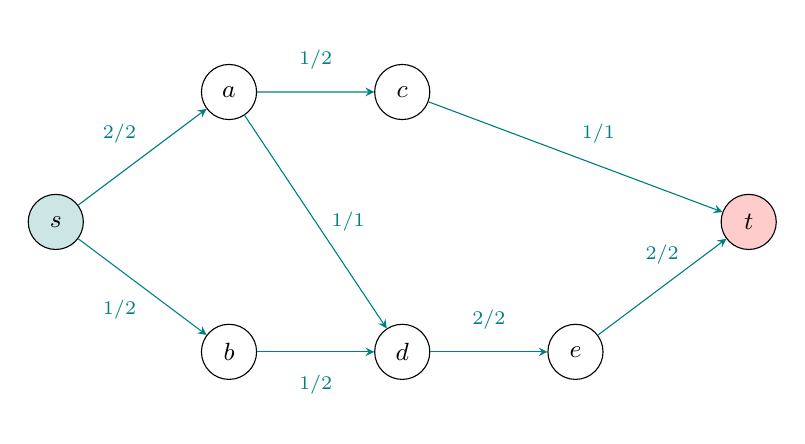
\begin{tikzpicture}[
  every node/.style={circle,draw,minimum size=0.7cm,font=\small},
  scale=1.1, ->, >=stealth
]
  \node[fill=teal!20]  (s) at (0,1.5)  {$s$};
  \node (a) at (2,3)    {$a$};
  \node (b) at (2,0)    {$b$};
  \node (c) at (4,3)    {$c$};
  \node (d) at (4,0)    {$d$};
  \node (e) at (6,0)  {$e$};
  \node[fill=red!20] (t) at (8,1.5)  {$t$};
 
  \draw[teal] (s)--node[draw=none,above left,font=\scriptsize]{2/2}(a);
  \draw[teal]              (s)--node[draw=none,below left,font=\scriptsize]{1/2}(b);
  \draw[teal]              (a)--node[draw=none,above,font=\scriptsize]{1/2}(c);
  \draw[teal] (a)--node[draw=none,right,font=\scriptsize]{1/1}(d);
  \draw[teal]              (b)--node[draw=none,below,font=\scriptsize]{1/2}(d);
  \draw[teal] (c)--node[draw=none,above right,font=\scriptsize]{1/1}(t);
  \draw[teal] (d)--node[draw=none,above,font=\scriptsize]{2/2}(e);
  \draw[teal] (e)--node[draw=none,above,font=\scriptsize]{2/2}(t);
\end{tikzpicture}
\end{figure}
Nótese que si quisiésemos hacer otra fase, el BFS ya no encontraría a $t$, por lo que el algoritmo concluye aquí. Para esta red el flujo máximo es $3$. Con esto ya podemos resolver el problema inicial de servidores.
\\\\
Nótese que como  la longitud máxima es $|V|-1$, hay a lo más $|V|-1$ fases. Cada fase cuesta $O(VE)$, dando complejidad total $O(V^2 E)$.
\begin{lstlisting}[language=C++]
const long long INF = 1e17;

struct FlowEdge {
    int u, v;
    long long cap, flow = 0;

    FlowEdge(int u, int v, long long cap) : u(u), v(v), cap(cap) {}
};

struct Dinic {
    vector<FlowEdge> edges;
    vector<vector<int>> adj;
    int n, s, t;
    int edgeId = 0;
    vector<int> level, next;
    queue<int> q;

    Dinic(int n, int s, int t) : n(n), s(s), t(t) {
        adj.resize(n);
        level.resize(n);
        next.resize(n);
        fill(level.begin(), level.end(), -1);
        level[s] = 0;
        q.push(s);
    }

    void add(int u, int v, long long cap) {
        edges.emplace_back(u, v, cap);   // arista directa
        edges.emplace_back(v, u, 0);     // arista residual inversa
        adj[u].push_back(edgeId++);
        adj[v].push_back(edgeId++);
    }

    // Construye el grafo de niveles en la red residual.
    bool bfs() {
        while (!q.empty()) {
            int u = q.front();
            q.pop();

            for (int e : adj[u]) {
                int v = edges[e].v;
                if (edges[e].cap - edges[e].flow < 1) {
                    continue;
                }
                if (level[v] != -1) {
                    continue;
                }
                level[v] = level[u] + 1;
                q.push(v);
            }
        }
        return level[t] != -1;
    }

    // Empuja flujo a lo largo de un camino de niveles s -> ... -> t.
    long long dfs(int u, long long pushed) {
        if (pushed == 0) {
            return 0;
        }
        if (u == t) {
            return pushed;
        }

        for (int& cid = next[u]; cid < (int)adj[u].size(); cid++) {
            int e = adj[u][cid];
            int v = edges[e].v;

            if (level[u] + 1 != level[v] || edges[e].cap - edges[e].flow < 1) {
                continue;
            }

            long long tr = dfs(v, min(pushed, edges[e].cap - edges[e].flow));
            if (tr == 0) {
                continue;
            }

            edges[e].flow += tr;
            edges[e ^ 1].flow -= tr;
            return tr;
        }
        return 0;
    }

    long long maxFlow() {
        long long flow = 0;

        while (bfs()) {
            fill(next.begin(), next.end(), 0);

            while (true) {
                long long pushed = dfs(s, INF);
                if (pushed == 0) {
                    break;
                }
                flow += pushed;
            }

            fill(level.begin(), level.end(), -1);
            level[s] = 0;
            q.push(s);
        }

        return flow;
    }
};
\end{lstlisting}
\subsection{Teorema max-flow min-cut}
\begin{definition} Un \textbf{corte $s$-$t$} es una división de los vértices de $V$ en dos partes $(S, T)$ con $s \in S$ y $t \in T$. La \textbf{capacidad del corte} es la suma de las capacidades de los cables que van de $S$ a $T$:
\[
\text{cap}(S,T) = \sum_{\substack{u \in S,\, v \in T \\ (u,v)\in E}} c(u,v)
\]
El \textbf{corte mínimo} es el de menor capacidad.
\end{definition}
Un teorema muy importante es el \textbf{Teorema de Flujo Máximo y Corte Mínimo} que nos dice que el valor del flujo máximo de $s$ a $t$ es igual a la capacidad del corte mínimo $s$-$t$\footnote{\url{https://www.cs.toronto.edu/~lalla/373s16/notes/MFMC.pdf}}.
\\\\
Después de correr Dinic, si hacemos BFS en el grafo residual desde $s$.
Los nodos alcanzables forman $S$ y los no alcanzables $T$. Los cables
saturados de $S$ a $T$ forman el corte mínimo.
\\\\
Este teorema tiene consecuencias directas que usaremos en la sección siguiente de matching.
\\\\
Una aplicación bonita que podemos darle es encontrar \textbf{caminos arista-disjuntos}, es decir, el número máximo de caminos de $s$ a
$t$ que no comparten aristas. Este problema se traduce en buscar el mínimo número de aristas cuyo corte desconecta $s$ de $t$. Se calcula dando capacidad 1 a cada arista y corriendo flujo máximo.
 
\subsection{Matching máximo}

Para motivar esta sección, veamos el siguiente problema, \href{https://vjudge.net/problem/UVA-11419}{SAM I AM}, en este problema, hay una cuadrícula $R \times C$ con $N$ enemigos en ciertas celdas. Un cañón dispara en línea recta y elimina a todos los enemigos de una fila o columna. ¿Cuál es la mínima cantidad de disparos que se necesitan para eliminar a todos los enemigos y qué filas o columnas hay que disparar?
\\\\Podríamos intentar una estrategia greedy, es decir, intentar disparar las filas o columnas que tengan más enemigos, pero veámos en el siguiente ejemplo que pueden existir situaciones en las que alguna fila y columna tengan el mismo número de enemigos y no dé lo mismo cuál quitar. La solución optima es disparar la columna $1$ y $3$. Sin embargo, nuestro algoritmo greedy no tiene forma de distinguir entre la fila $1$ y las columnas $1$ y $3$ entonces podría iniciar disparando la fila $1$ y después, las filas $1$ y $3$, gastando $3$ disparos.

\begin{figure}[H]
\centering
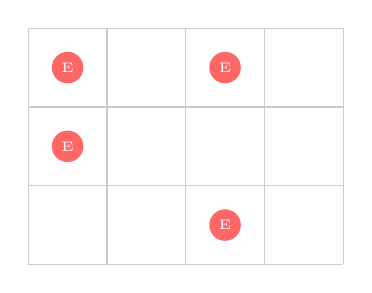
\begin{tikzpicture}[scale=1.0]
    \begin{scope}
    \draw[gray!40] (0,0) grid (4,3);
    \fill[red!60] (0.5,2.5) circle (0.2) node[white, font=\tiny] {E};
    \fill[red!60] (2.5,2.5) circle (0.2) node[white, font=\tiny] {E};
    \fill[red!60] (0.5,1.5) circle (0.2) node[white, font=\tiny] {E};
    \fill[red!60] (2.5,0.5) circle (0.2) node[white, font=\tiny] {E};
  \end{scope}
\end{tikzpicture}
\end{figure}

Necesitamos otra forma de pensar el problema. Podemos intentar modelarlo como una gráfica bipartita, este pensamiento surge de la idea que cada enemigo es cubierto si disparamos la fila $r$ \textbf{o} la columna $c$.
 
\begin{itemize}
    \item Lado izquierdo, un vértice por cada fila ($R$ vértices)
    \item Lado derecho, un vértice por cada columna ($C$ vértices)
    \item Por cada enemigo en $(r,c)$, una arista entre la fila $r$ y la columna $c$
\end{itemize}
 
\begin{figure}[H]
\centering
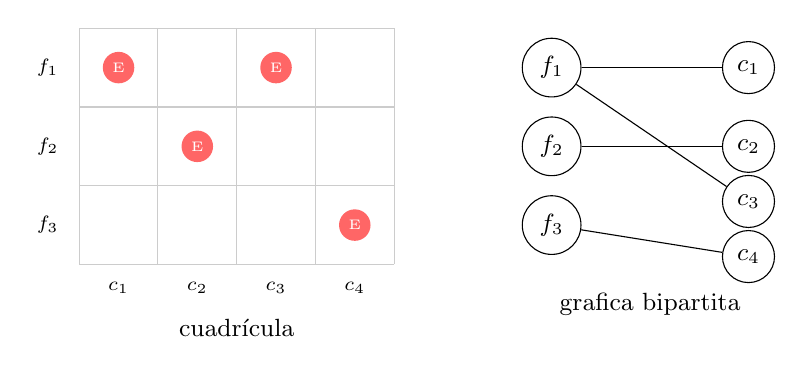
\begin{tikzpicture}[scale=1.0]
  \begin{scope}
    \draw[gray!40] (0,0) grid (4,3);
    \fill[red!60] (0.5,2.5) circle (0.2) node[white, font=\tiny] {E};
    \fill[red!60] (2.5,2.5) circle (0.2) node[white, font=\tiny] {E};
    \fill[red!60] (1.5,1.5) circle (0.2) node[white, font=\tiny] {E};
    \fill[red!60] (3.5,0.5) circle (0.2) node[white, font=\tiny] {E};
    \node[font=\scriptsize] at (-0.4, 2.5) {$f_1$};
    \node[font=\scriptsize] at (-0.4, 1.5) {$f_2$};
    \node[font=\scriptsize] at (-0.4, 0.5) {$f_3$};
    \node[font=\scriptsize] at (0.5, -0.3) {$c_1$};
    \node[font=\scriptsize] at (1.5, -0.3) {$c_2$};
    \node[font=\scriptsize] at (2.5, -0.3) {$c_3$};
    \node[font=\scriptsize] at (3.5, -0.3) {$c_4$};
    \node[font=\small] at (2, -0.8) {cuadrícula};
  \end{scope}
 
  \begin{scope}[xshift=6cm]
    \node[circle, draw, minimum size=0.6cm, font=\small] (f1) at (0, 2.5) {$f_1$};
    \node[circle, draw, minimum size=0.6cm, font=\small] (f2) at (0, 1.5) {$f_2$};
    \node[circle, draw, minimum size=0.6cm, font=\small] (f3) at (0, 0.5) {$f_3$};
    \node[circle, draw, minimum size=0.6cm, font=\small] (c1) at (2.5, 2.5) {$c_1$};
    \node[circle, draw, minimum size=0.6cm, font=\small] (c2) at (2.5, 1.5) {$c_2$};
    \node[circle, draw, minimum size=0.6cm, font=\small] (c3) at (2.5, 0.8) {$c_3$};
    \node[circle, draw, minimum size=0.6cm, font=\small] (c4) at (2.5, 0.1) {$c_4$};
    \draw (f1)--(c1); 
    \draw (f1)--(c3);  
    \draw (f2)--(c2); 
    \draw (f3)--(c4);  
    \node[font=\small] at (1.25, -0.5) {grafica bipartita};
  \end{scope}
\end{tikzpicture}
\end{figure}

Nótese entonces que queremos seleccionar un conjunto de vértices $S$ de forma que cualquier arista tenga al menos un extremo en $S$, a esto se le llama \textbf{cobertura de vértices}. Queremos entonces la cobertura de menor tamaño, en gráficas generales este problema es $NP$, pero en gráficas bipartitas como esta resulta que la clave para resolver el problema es usar flujo máximo.
\\\\Esto puede parecer raro porque la gráfica que construimos no parece indicar por ningún lado un flujo, pero podemos cosntruir la red agregando un nodo $s$ conectado a cada fila y un nodo $t$ conectado a cada columna. A todas las aristas les pondremos capacidad $1$.
\begin{figure}[H]
\centering
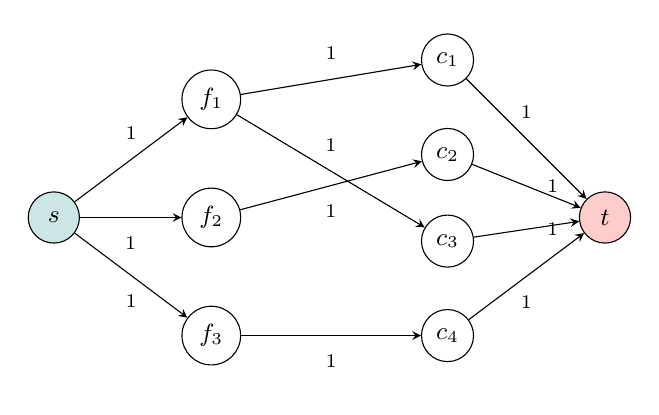
\begin{tikzpicture}[
  every node/.style={circle,draw,minimum size=0.65cm,font=\small},
  scale=1.0, ->, >=stealth
]
  \node[fill=teal!20]  (s)  at (0,1.5)  {$s$};
  \node (f1) at (2,3)    {$f_1$};
  \node (f2) at (2,1.5)  {$f_2$};
  \node (f3) at (2,0)    {$f_3$};
  \node (c1) at (5,3.5)  {$c_1$};
  \node (c2) at (5,2.3)  {$c_2$};
  \node (c3) at (5,1.2)  {$c_3$};
  \node (c4) at (5,0)    {$c_4$};
  \node[fill=red!20] (t)  at (7,1.5)  {$t$};
 
  \draw (s)--node[draw=none,above,font=\scriptsize]{1}(f1);
  \draw (s)--node[draw=none,below,font=\scriptsize]{1}(f2);
  \draw (s)--node[draw=none,below,font=\scriptsize]{1}(f3);
  \draw (f1)--node[draw=none,above,font=\scriptsize]{1}(c1);
  \draw (f1)--node[draw=none,above,font=\scriptsize]{1}(c3);
  \draw (f2)--node[draw=none,below,font=\scriptsize]{1}(c2);
  \draw (f3)--node[draw=none,below,font=\scriptsize]{1}(c4);
  \draw (c1)--node[draw=none,above,font=\scriptsize]{1}(t);
  \draw (c2)--node[draw=none,right,font=\scriptsize]{1}(t);
  \draw (c3)--node[draw=none,right,font=\scriptsize]{1}(t);
  \draw (c4)--node[draw=none,below,font=\scriptsize]{1}(t);
\end{tikzpicture}
\end{figure}
Si corremos Dinic en esta red, el flujo máximo resulta ser 3, que es
exactamente el número mínimo de disparos que necesitamos. ¿Casualidad? Como veremos en esta sección, no lo es.

\begin{definition}Un \textbf{matching} es un subconjunto de aristas tal que ningún vértice es extremo de más de una arista. El \textbf{matching máximo} es el de mayor cardinalidad.
\end{definition}
 
Traducido al problema que estamos resolviendo, un matching en nuestra gráfica es un conjunto de enemigos tal que no hay dos en la misma fila ni en la misma columna. El matching máximo es el mayor conjunto así.
 
\begin{figure}[H]
\centering
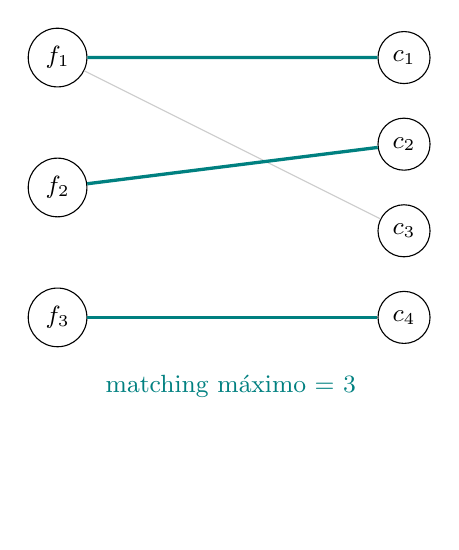
\begin{tikzpicture}[
  every node/.style={circle,draw,minimum size=0.65cm,font=\small},
  scale=1.1
]
  \node (f1) at (0,3)   {$f_1$};
  \node (f2) at (0,1.5) {$f_2$};
  \node (f3) at (0,0)   {$f_3$};
  \node (c1) at (4,3)   {$c_1$};
  \node (c2) at (4,2)   {$c_2$};
  \node (c3) at (4,1)   {$c_3$};
  \node (c4) at (4,0)   {$c_4$};
 
  \draw[gray!40] (f1)--(c1);
  \draw[gray!40] (f1)--(c3);
  \draw[gray!40] (f2)--(c2);
  \draw[gray!40] (f3)--(c4);
  \draw[teal,very thick] (f1)--(c1);
  \draw[teal,very thick] (f2)--(c2);
  \draw[teal,very thick] (f3)--(c4);
  \node[draw=none,font=\small,teal] at (2,-0.8) {matching máximo = 3};
\end{tikzpicture}
\end{figure}

\subsection*{Hopcroft-Karp: Dinic en bipartitos}
 
El matching máximo en una gráfica bipartita se puede calcular directamente
con la red de flujo anterior usando Dinic. Pero como esta gráfica tiene
estructura especial (bipartito, todas las capacidades 1), se puede
optimizar, el algoritmo \textbf{Hopcroft-Karp} es exactamente Dinic
aplicado a gráficas bipartitos, con complejidad $O(E\sqrt{V})$ en lugar
de $O(V^2 E)$.
 
\begin{lstlisting}[language=C++]
const int INF = 1e9;
int n, m;                           // |L| = n, |R| = m
vector<int> adj[MAXN];              // adj[u] = vecinos de u (lado izquierdo)
int matchL[MAXN], matchR[MAXN];    // emparejamiento actual
int dist[MAXN];

// Construye capas de caminos aumentantes disjuntos.
bool bfs() {
    queue<int> q;
    for (int u = 1; u <= n; u++) {
        if (!matchL[u]) {
            dist[u] = 0;
            q.push(u);
        } else {
            dist[u] = INF;
        }
    }

    bool found = false;
    while (!q.empty()) {
        int u = q.front();
        q.pop();

        for (int v : adj[u]) {
            int w = matchR[v];
            if (!w) {
                found = true;  // camino aumentante libre
            } else if (dist[w] == INF) {
                dist[w] = dist[u] + 1;
                q.push(w);
            }
        }
    }
    return found;
}

// Intenta aumentar el matching desde u siguiendo las capas de BFS.
bool dfs(int u) {
    for (int v : adj[u]) {
        int w = matchR[v];
        if (!w || (dist[w] == dist[u] + 1 && dfs(w))) {
            matchL[u] = v;
            matchR[v] = u;
            return true;
        }
    }
    dist[u] = INF;
    return false;
}

int hopcroftKarp() {
    fill(matchL + 1, matchL + n + 1, 0);
    fill(matchR + 1, matchR + m + 1, 0);

    int matching = 0;
    while (bfs()) {
        for (int u = 1; u <= n; u++) {
            if (!matchL[u] && dfs(u)) {
                matching++;
            }
        }
    }
    return matching;
}
\end{lstlisting}

\subsection{Teorema de König}
El \textbf{teorema de König} nos dice que en una gráfica bipartita el matching máximo es igual a la cobertura mínima de vértices\footnote{\url{https://www.math.nagoya-u.ac.jp/~richard/teaching/s2024/SML_Li_2.pdf}}.
\\\\
Veámos la red del problema de los cañones. El flujo máximo = matching
máximo (cada unidad de flujo es un par emparejado). El corte mínimo =
cubierta mínima (los vértices del corte son exactamente las
filas/columnas que hay que disparar). Por el teorema anterior, son lo mismo, entonces calculado el flujo máximo, ¿cómo construir la cubierta mínima?
Supongamos que tenemos esta cuadrícula con los enemigos:
\begin{figure}[H]
\centering
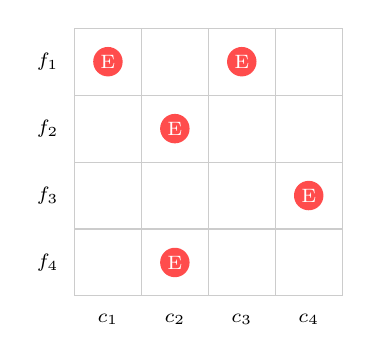
\begin{tikzpicture}[scale=0.85]
  \draw[gray!40] (0,0) grid (4,4);
  \fill[red!70] (0.5,3.5) circle (0.22) node[white,font=\scriptsize]{E};
  \fill[red!70] (2.5,3.5) circle (0.22) node[white,font=\scriptsize]{E};
  \fill[red!70] (1.5,2.5) circle (0.22) node[white,font=\scriptsize]{E};
  \fill[red!70] (3.5,1.5) circle (0.22) node[white,font=\scriptsize]{E};
  \fill[red!70] (1.5,0.5) circle (0.22) node[white,font=\scriptsize]{E};
  \node[font=\scriptsize] at (-0.4,3.5) {$f_1$};
  \node[font=\scriptsize] at (-0.4,2.5) {$f_2$};
  \node[font=\scriptsize] at (-0.4,1.5) {$f_3$};
  \node[font=\scriptsize] at (-0.4,0.5) {$f_4$};
  \node[font=\scriptsize] at (0.5,-0.35) {$c_1$};
  \node[font=\scriptsize] at (1.5,-0.35) {$c_2$};
  \node[font=\scriptsize] at (2.5,-0.35) {$c_3$};
  \node[font=\scriptsize] at (3.5,-0.35) {$c_4$};
\end{tikzpicture}
\hspace{1.5cm}
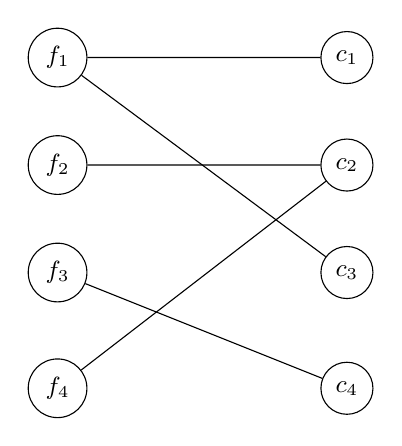
\begin{tikzpicture}[
  every node/.style={circle,draw,minimum size=0.65cm,font=\small},
  scale=1.05
]
  \node (f1) at (0,4)   {$f_1$};
  \node (f2) at (0,2.7) {$f_2$};
  \node (f3) at (0,1.4) {$f_3$};
  \node (f4) at (0,0)   {$f_4$};
  \node (c1) at (3.5,4)   {$c_1$};
  \node (c2) at (3.5,2.7) {$c_2$};
  \node (c3) at (3.5,1.4) {$c_3$};
  \node (c4) at (3.5,0)   {$c_4$};
  \draw (f1)--(c1); \draw (f1)--(c3);
  \draw (f2)--(c2); \draw (f3)--(c4); \draw (f4)--(c2);
\end{tikzpicture}
\end{figure}

Podemos usar Hopcroft-Karp o Dinic para encontrar el matching máximo de tamaño 3 con las aristas:
$f_1\text{-}c_1,\ f_2\text{-}c_2,\ f_3\text{-}c_4$.
\\\\
Lo siguiente que haremos, será partir desde cada vértice libre del lado izquierdo, en este caso solo tenemos $f_4$ y alternar aristas fuera/dentro del matching. En la figura de abajo, usamos $f_4\to c_2$ que está fuera del matching, luego $c_2\to f_2$ que está dentro del matching y ya no tenemos a dónde movernos pues $c_2\to f_2$ ya fue visitada.
 
\begin{figure}[H]
\centering
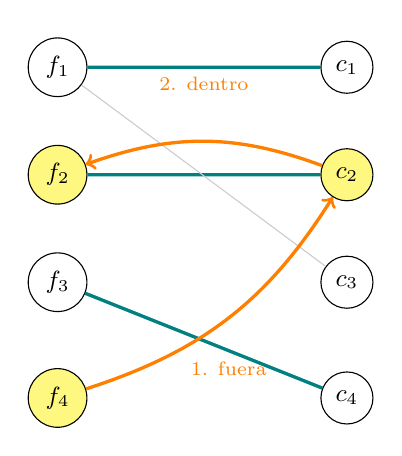
\begin{tikzpicture}[
  every node/.style={circle,draw,minimum size=0.65cm,font=\small},
  scale=1.05
]
  \node (f1) at (0,4)   {$f_1$};
  \node[fill=yellow!50] (f2) at (0,2.7) {$f_2$};
  \node (f3) at (0,1.4) {$f_3$};
  \node[fill=yellow!50] (f4) at (0,0)   {$f_4$};
  \node (c1) at (3.5,4)   {$c_1$};
  \node[fill=yellow!50] (c2) at (3.5,2.7) {$c_2$};
  \node (c3) at (3.5,1.4) {$c_3$};
  \node (c4) at (3.5,0)   {$c_4$};
 
  \draw[teal,very thick] (f1)--(c1);
  \draw[teal,very thick] (f2)--(c2);
  \draw[teal,very thick] (f3)--(c4);
  \draw[gray!40] (f1)--(c3);
 
  \draw[orange,very thick,->] (f4) to[bend right=20]
    node[draw=none,below,font=\scriptsize,orange]{1. fuera}(c2);
  \draw[orange,very thick,->] (c2) to[bend right=20]
    node[draw=none,above,font=\scriptsize,orange]{2. dentro}(f2);
\end{tikzpicture}
\end{figure}

Ahora, para constuir la cubierta usaremos estos vértices que marcamos (los que quedaron en amarillo), la cubierta mínima se forma con:
\begin{itemize}
    \item Los vértices del lado \textbf{izquierdo no marcados}
    \item Los vértices del lado \textbf{derecho marcados}
\end{itemize}
\begin{center}
\begin{tabular}{lcc}
\toprule
Vértice & Marcado & ¿En la cubierta? \\
\midrule
$f_1$ & No  & \textbf{Sí} (izq no marcada) \\
$f_2$ & Sí  & No \\
$f_3$ & No  & \textbf{Sí} (izq no marcada) \\
$f_4$ & Sí  & No \\
$c_1$ & No  & No \\
$c_2$ & Sí  & \textbf{Sí} (drch marcada) \\
$c_3$ & No  & No \\
$c_4$ & No  & No \\
\bottomrule
\end{tabular}
\end{center}
 De forma que la cubierta mínima es de tamaño $3$ y consiste en $\{f_1,\ f_3,\ c_2\}$.
 
\begin{figure}[H]
\centering
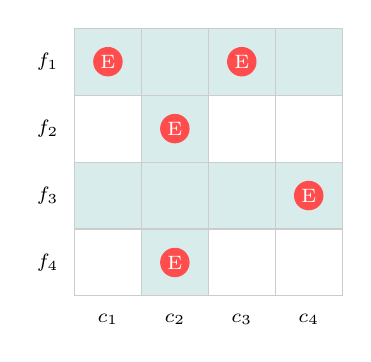
\begin{tikzpicture}[scale=0.85]
  \draw[gray!40] (0,0) grid (4,4);
  \fill[teal!15] (0,3) rectangle (4,4);   
  \fill[teal!15] (0,1) rectangle (4,2);   
  \fill[teal!15] (1,0) rectangle (2,4);   
  \draw[gray!40] (0,0) grid (4,4);
  \fill[red!70] (0.5,3.5) circle (0.22) node[white,font=\scriptsize]{E};
  \fill[red!70] (2.5,3.5) circle (0.22) node[white,font=\scriptsize]{E};
  \fill[red!70] (1.5,2.5) circle (0.22) node[white,font=\scriptsize]{E};
  \fill[red!70] (3.5,1.5) circle (0.22) node[white,font=\scriptsize]{E};
  \fill[red!70] (1.5,0.5) circle (0.22) node[white,font=\scriptsize]{E};
  \node[font=\scriptsize] at (-0.4,3.5) {$f_1$};
  \node[font=\scriptsize] at (-0.4,2.5) {$f_2$};
  \node[font=\scriptsize] at (-0.4,1.5) {$f_3$};
  \node[font=\scriptsize] at (-0.4,0.5) {$f_4$};
  \node[font=\scriptsize] at (0.5,-0.35) {$c_1$};
  \node[font=\scriptsize] at (1.5,-0.35) {$c_2$};
  \node[font=\scriptsize] at (2.5,-0.35) {$c_3$};
  \node[font=\scriptsize] at (3.5,-0.35) {$c_4$};
\end{tikzpicture}
\end{figure}

\textbf{Ejercicio.} Completar la solución del problema \href{https://vjudge.net/problem/UVA-11419}{SAM I AM}.

\subsection{Teorema de Hall}
Una pregunta natural que podría surgir es ¿cuándo existe un matching que empareja \textbf{todos} los vértices de un lado?
\\\\
En un grafo bipartito con lados $L$ y $R$, existe un matching que
empareja todos los vértices de $L$ si y solo si para todo
$S \subseteq L$:
\[
|N(S)| \geq |S|
\]
donde $N(S)$ es el conjunto de vecinos de $S$ en $R$.
 
\begin{figure}[H]
\centering
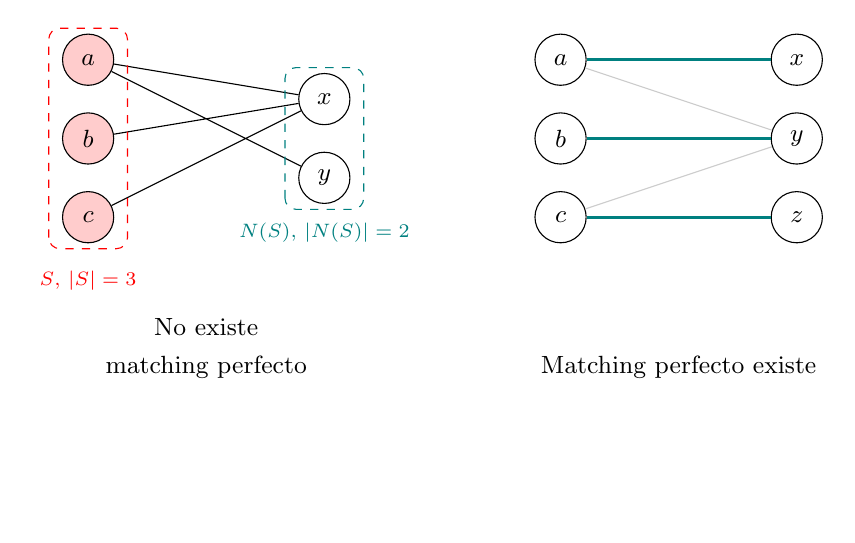
\begin{tikzpicture}[
  every node/.style={circle,draw,minimum size=0.65cm,font=\small},
  scale=1.0
]
  \begin{scope}
    \node[fill=red!20] (a) at (0,3) {$a$};
    \node[fill=red!20] (b) at (0,2) {$b$};
    \node[fill=red!20] (c) at (0,1) {$c$};
    \node (x) at (3,2.5) {$x$};
    \node (y) at (3,1.5) {$y$};
    \draw (a)--(x) (a)--(y) (b)--(x) (c)--(x);
    \draw[red,dashed,rounded corners] (-0.5,0.6) rectangle (0.5,3.4);
    \draw[teal,dashed,rounded corners]  (2.5,1.1) rectangle (3.5,2.9);
    \node[draw=none,red,font=\scriptsize] at (0,0.2)  {$S$, $|S|=3$};
    \node[draw=none,teal,font=\scriptsize]  at (3,0.8)  {$N(S)$, $|N(S)|=2$};
    \node[draw=none,font=\small] at (1.5,-0.4) {No existe};
    \node[draw=none,font=\small] at (1.5,-0.9) {matching perfecto};
  \end{scope}
 
  \begin{scope}[xshift=6cm]
    \node (a2) at (0,3) {$a$};
    \node (b2) at (0,2) {$b$};
    \node (c2) at (0,1) {$c$};
    \node (x2) at (3,3) {$x$};
    \node (y2) at (3,2) {$y$};
    \node (z2) at (3,1) {$z$};
    \draw[gray!40] (a2)--(x2) (a2)--(y2) (b2)--(y2) (c2)--(y2) (c2)--(z2);
    \draw[teal,very thick] (a2)--(x2) (b2)--(y2) (c2)--(z2);
    \node[draw=none,font=\small] at (1.5,-0.9) {Matching perfecto existe};
  \end{scope}
\end{tikzpicture}
\end{figure}
\subsection*{Matching de peso mínimo}
Cuando las aristas tienen pesos y queremos el matching perfecto de costo
mínimo (o máximo), se usa el \textbf{algoritmo Húngaro} (Kuhn-Munkres),
con complejidad $O(n^3)$. Aparece en problemas de asignación óptima: dados
$n$ trabajadores, $n$ tareas, y costos $c_{ij}$ de asignar el trabajador
$i$ a la tarea $j$, minimizar el costo total. La mejor referencia que he encontrado para este algoritmo es \url{https://www.topcoder.com/thrive/articles/Assignment%20Problem%20and%20Hungarian%20Algorithm}.

\section{Ejercicios}
\subsection*{9.10.1 \href{https://codeforces.com/problemset/problem/808/F}{Card Game (Codeforces)}}

\textbf{Descripción: }\url{https://codeforces.com/problemset/problem/808/F}

Si un conjunto de cartas con $l_i \leq L$ permite alcanzar potencia $\geq k$, entonces
también lo permite cualquier nivel mayor (hay más cartas disponibles). Podemos hacer búsqueda binaria sobre el nivel necesario.

Dado un nivel $L$, construimos una gráfica $G$ donde cada carta disponible (con $l_i \leq L$) es un vértice, con peso $p_i$, y conectamos dos
cartas $i,j$ con una arista si $c_i+c_j$ es primo es decir, si no pueden estar juntas en el mazo. Un subconjunto $S$ es un mazo válido si y solo si $S$ es un conjunto independiente en $G$ (no contiene ninguna arista).

Sea $P$ la suma de potencias de todas las cartas disponibles (con $l_i \leq L$). Buscamos un subconjunto $S$ sin pares prohibidos con $\sum_{i\in S} p_i \geq k$. Esto es equivalente a encontrar el conjunto descartado $D = V\setminus S$ de peso mínimo  tal que $D$ sea una cobertura de vértices de todas las aristas prohibidas, es decir, toda pareja prohibida tiene al menos un extremo en $D$ (así $S$ queda libre de conflictos). La condición para verificar que es un conjunto válido es
$P - \text{peso}(D) \geq k$.
 
Por el teorema de König, la covertura de vértices de peso mínimo en una gráfica bipartita es igual al matching máximo.
 
Notemos que si $c_i+c_j$ es un primo mayor que 2, entonces $c_i+c_j$ es impar, así que $c_i$ y $c_j$ tienen paridades distintas. Esto
sugiere separar las cartas en dos grupos — pares e impares y las aristas prohibidas solo conectarían cartas de grupos distintos, dando un gráfica bipartita.
 
Lo anterior tiene un caso especial si $c_i=1$, pues el único primo par es 2, y $1+1=2$. Entonces dos cartas con $c_i=c_j=1$ son
mutuamente prohibidas, pero ambas caen en el lado "impar", haciendo que la gráfica no sea bipartita. Para solucionar esto, notemos que si tomamos dos o más cartas con $c=1$, hay
un par prohibido entre ellas siempre. Por lo
tanto, en el conjunto óptimo $S$, a lo más puede haber una carta con $c=1$. Por lo que para cada $L$, si hubiera varias cartas con $c=1$ disponibles, tomaremos la de mayor potencia.
 
Sean $A$ las cartas con $c_i$ impar, y $B$ las
cartas con $c_i$ par disponibles con nivel $L$:
 
\begin{itemize}
    \item \textbf{Fuente $\to$ carta} $\in A$, con capacidad $p_i$.
    \item \textbf{Carta} $j \in B \to$ \textbf{Sumidero}, con capacidad $p_j$.
    \item \textbf{Carta} $i \to$ \textbf{Carta} $j$ (impar a par), con capacidad $\infty$, si $c_i+c_j$ es primo.
\end{itemize}
 
Un corte finito en esta red nunca incluye aristas $\infty$ (impar$\to$par), esas aristas garantizan que si una carta impar $i$ y una carta par $j$ tienen $c_i+c_j$ primo, al menos
una de las dos aristas (fuente$\to i$ o $j\to$sumidero) debe estar en el corte. Es decir, el corte mínimo identifica exactamente el conjunto $D$ de cartas a descartar con peso mínimo que rompe todas las parejas prohibidas. Por max-flow = min-cut, basta entonces calcular el maxFlow de la gráfica construida y ver si:
\[
P - \text{maxFlow} \geq k
\]
 
La complejidad es $O(\log n)$ para las iteraciones de búsqueda binaria, cada una con un max flow en una red de $O(n)$ nodos y $O(n^2)$ aristas.

Ver \codelink{https://codeforces.com/contest/808/submission/273807670}.

\subsection*{9.10.2 \href{https://www.spoj.com/problems/QTREE2/}{Query on a tree III (SPOJ)}}

\textbf{Descripción: }\url{https://www.spoj.com/problems/QTREE2/}

 Para resolver el primer tipo de consulta notemos que el camino de $a$ a $b$ pasa por su LCA $L$, y se descompone en el camino $a \to L$ más el camino $L \to b$. Si guardamos para cada vértice la distancia acumulada desde la raíz
(\texttt{distRoot}), entonces:
\[
\text{dist}(a,b) = \text{distRoot}(a) + \text{distRoot}(b) -
2\cdot\text{distRoot}(L)
\]
La resta de $2\cdot\text{distRoot}(L)$ elimina el camino duplicado desde la raíz hasta $L$, que está contado una vez en $\text{distRoot}(a)$ y otra vez en $\text{distRoot}(b)$.
 
Para el segundo tipo de consulta, veamos que el camino de $a$ a $b$ (en número de vértices) se compone de dos partes, el camino $a \to L$, con $\text{depth}(a) - \text{depth}(L) + 1$ vértices (incluyendo $a$ y $L$), y del camino $L \to b$ (sin repetir $L$), con $\text{depth}(b) - \text{depth}(L)$ vértices adicionales.
 
Sea $\text{len}_A = \text{depth}(a) - \text{depth}(L)$ (número
de \textbf{aristas} de $a$ a $L$).
 
\begin{itemize}
    \item Si $k-1 \leq \text{depth}(a)- \text{depth}(L)$:
    
          El $k$-ésimo vértice está en el camino $a \to L$, a $k-1$ aristas de
          distancia de $a$ hacia arriba, es decir es el $(k-1)$-ésimo ancestro de $a$.
 
    \item En caso contrario:
    
          El $k$-ésimo nodo está en el camino
          $L \to b$. El nodo está a:
          \[\text{s} = dist(a,b)-(k-1)\]
          aristas de distancia de $b$ hacia arriba, es decir, el $\text{s}$-ésimo ancestro de $b$.
\end{itemize}
 Para ambos casos es eficiente recuperar el ancestro con binary lifting (la técnica de descomponer los niveles que queremos subir en potencias de dos).

 Ver \codelink{https://github.com/MelitoMT/ICPC_Manual/tree/master/tex/codes/editorial/qtree2.cpp}.

\section{Problemas}
\begin{itemize}
  \item[9.11.1] \href{https://cses.fi/problemset/task/2079}{Finding a Centroid (Codeforces 2079)}
  \item[9.11.2] \href{https://codeforces.com/group/DH4HPwQlLU/contest/689800/problem/I}{Zuko vs Aang (Autoría $\filledstar$)}
  \item[9.11.3] \href{https://codeforces.com/problemset/problem/652/E}{Pursuit for artifacts (Codeforces 652E)}
  \item[9.11.4] \href{https://codeforces.com/contest/1404/problem/E}{Bricks (Codeforces 1404E)}
\end{itemize}